\subsection{\texorpdfstring{\(\tau\)-扩张的直像}{\textbackslash tau-扩张的直像}}

设 G 是一个群，设 F 与 \(F'\) 是交换群，设 \(\tau\)（相应地，\(\tau'\)）是一个群同态（从 G 到 F（相应地，\(F'\)）的自同构群的），并设 \(v: F \to F'\) 是一个群同态，使得

\[
v (\tau (g) \cdot f) = \tau^ {\prime} (g) \cdot v (f)\tag{3}
\]

（对每个 \(g \in G\) 与 \(f \in F\)）。设 \(\mathcal{E} = (\Gamma, \iota, \pi)\) 是 G 被 F 的一个 \(\tau\)-扩张。设 \(\widetilde{\Gamma}\) 是外半直积 \(F' \times_{\tau' \circ \pi} \Gamma\)。用 \(\widetilde{\iota}: F' \to \widetilde{\Gamma}\) 表示同态 \(f \mapsto (f, e)\)，并用 \(\widetilde{p}: \widetilde{\Gamma} \to \Gamma\) 表示第一个投影。设 \(j: F \to \widetilde{\Gamma}\) 是由 \(f \mapsto (v(f), \iota(f)^{-1})\) 定义的映射。由于 \(\iota\) 的像包含在 \(\tau' \circ \pi\) 的核中，映射 j 是一个群同态；由于 \(\iota\) 是单射的，它是单射的。我们有关系

\[
\begin{array}{r l} (f ^ {\prime}, \gamma) j (f) (f ^ {\prime}, \gamma) ^ {- 1} & = (f ^ {\prime}, \gamma) (v (f), \iota (f) ^ {- 1}) (f ^ {\prime}, \gamma) ^ {- 1} \\ & = (\tau^ {\prime} (\pi (\gamma)) \cdot v (f), \iota (\tau (\pi (\gamma)) \cdot f) ^ {- 1}) \\ & = j (\tau (\pi (\gamma)) \cdot f) \end{array}\tag{4}
\]

（对 \(f \in F\)、\(\gamma \in \Gamma\) 与 \(f' \in F'\)）。因此，j 的像是 \(\widetilde{\Gamma}\) 的一个正规子群。用 \(\Gamma'\) 表示 \(\widetilde{\Gamma}\) 关于 j 的像的商。用 \(\iota'\) 表示从 \(\widetilde{\Gamma}\) 到 \(\Gamma'\) 的典范满射与 \(\widetilde{\iota}\) 的复合。同态 \(\pi \circ \widetilde{p}\) 的核是积 \(\mathrm{F}' \times \iota(\mathrm{F})\)，它包含 j 的像。我们把 \(\pi' : \Gamma' \to G\) 定义为由 \(\pi \circ \widetilde{p}\) 通过过渡到商得到的群同态。由于 \(\iota\) 是单射的，\(j(\mathrm{F})\) 与 \(\widetilde{\iota}(\mathrm{F}')\) 的交化归为 \(\widetilde{\Gamma}\) 的单位元素；由此推出 \(\iota'\) 是单射的。从 \(F' \times F\) 到 \(F' \times \iota(\mathrm{F}) = \operatorname{Ker}(\pi \circ \widetilde{p})\) 的由

\[
(f ^ {\prime}, f) \longmapsto (f ^ {\prime} v (f), \iota (f) ^ {- 1})
\]

给出的映射是一个群同构。于是 \(\iota'\) 的像与 \(\pi'\) 的核重合。由于 \(\pi\) 与 \(\widetilde{p}\) 是满射的，\(\pi'\) 也是满射的。这就证明了 \(\mathcal{E}' = (\Gamma', \iota, \pi')\) 是一个 \(\tau'\)-扩张（\(G\) 被 \(F'\) 的）；我们称它为 \(\mathcal{E}\) 被 \(v\) 的直像，并记作 \(v_{*}(\mathcal{E})\)。从 \(\widetilde{\Gamma}\) 到 \(\Gamma'\) 的典范满射与从 \(\Gamma\) 到 \(\widetilde{\Gamma}\) 的由 \(\gamma \mapsto (1, \gamma)\) 给出的群同态的复合是一个群同态 \(\varphi : \Gamma \to \Gamma'\)，我们称之为典范的。

命题 2. —— 用上面的记号，下面的图交换：

\begin{enumerate}
\def\labelenumi{(\arabic{enumi})}
\setcounter{enumi}{4}
\tightlist
\item
\end{enumerate}

\pandocbounded{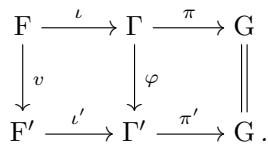
\includegraphics[keepaspectratio]{images/part002_f3abcdb3.jpg}}

设 \(\mathcal{E}_1' = (\Gamma_1', \iota_1', \pi_1')\) 是一个 \(\tau'\)-扩张（G 被 F' 的），并设 \(\varphi_1: \Gamma \to \Gamma_1'\) 是一个使得下图交换的群同态：

\pandocbounded{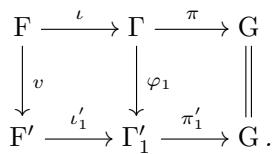
\includegraphics[keepaspectratio]{images/part002_c84edb93.jpg}}

则存在唯一的态射 \(\psi\)（\(\tau'\)-扩张的、从 \(v_{*}(\mathcal{E})\) 到 \(\mathcal{E}_1'\) 的），使得我们有 \(\varphi_1 = \psi \circ \varphi\)。

第一个图的交换性由构造得出。\(\psi\) 的存在性与唯一性由下面的引理 3 得出。

引理 3. —— 设 \(G_{1}^{\prime}\) 是一个群，并设 \(w: G \to G_{1}^{\prime}\) 与 \(\tau_{1}: G_{1}^{\prime} \to \operatorname{Aut}(F^{\prime})\) 是满足 \(\tau^{\prime} = \tau_{1} \circ w\) 的群同态。设 \(\mathcal{E}_{1}^{\prime} = (\Gamma_{1}^{\prime}, \iota_{1}^{\prime}, \pi_{1}^{\prime})\) 是一个 \(\tau_{1}\)-扩张（\(G_{1}^{\prime}\) 被 \(F^{\prime}\) 的），并设 \(\varphi_{1}: \Gamma \to \Gamma_{1}^{\prime}\) 是一个使得下图交换的群同态：

\[
\begin{array}{c} \mathrm{F} \xrightarrow {\iota} \Gamma \xrightarrow {\pi} \mathrm{G} \\ \Biggl \downarrow_ {v} \qquad \qquad \Biggl \downarrow_ {\varphi_ {1}} \qquad \Biggl \downarrow_ {w} \\ \mathrm{F} ^ {\prime} \xrightarrow {\iota_ {1} ^ {\prime}} \Gamma_ {1} ^ {\prime} \xrightarrow {\pi_ {1} ^ {\prime}} \mathrm{G} _ {1} ^ {\prime}. \end{array}
\]

则存在唯一的群同态 \(\psi : \Gamma' \to \Gamma'_1\)，使得图

\[
\begin{array}{c} \mathrm{F} ^ {\prime} \xrightarrow {\iota^ {\prime}} \Gamma^ {\prime} \xrightarrow {\pi^ {\prime}} \mathrm{G} \\ \Big \| \qquad \qquad \qquad \Big \downarrow_ {\psi} \qquad \Big \downarrow_ {w} \\ \mathrm{F} ^ {\prime} \xrightarrow {\iota_ {1} ^ {\prime}} \Gamma_ {1} ^ {\prime} \xrightarrow {\pi_ {1} ^ {\prime}} \mathrm{G} _ {1} ^ {\prime} \end{array}
\]

交换且 \(\varphi_{1} = \psi \circ \varphi\)。

对任何 \((f,\gamma)\in\mathrm{F}^{\prime}\times\Gamma\)，把 \((f,\gamma)\) 在 \(\Gamma^{\prime}\) 中的类记作 \(\overline{(f,\gamma)}\)。若群同态 \(\psi:\Gamma^{\prime}\to\Gamma_{1}^{\prime}\) 具有所要的性质，则它满足关系

\[
\psi \big (\overline {{(f ^ {\prime} , \gamma)}} \big) = \psi (\iota^ {\prime} (f ^ {\prime}) \varphi (\gamma)) = \iota_ {1} ^ {\prime} (f ^ {\prime}) \varphi_ {1} (\gamma)
\]

（对每个 \(f' \in \mathrm{F}'\) 与 \(\gamma \in \Gamma\)）。反之，映射 \(\tilde{\psi}\) 从 \(\mathrm{F}' \times_{\tau' \circ \pi} \Gamma\) 到 \(\Gamma_1'\) 由 \((f, \gamma) \mapsto \iota_1'(f) \varphi_1(\gamma)\) 给出，是一个群同态。实际上，我们有关系

\[
\begin{array}{r} \iota_ {1} ^ {\prime} (f) \varphi_ {1} (\gamma) \iota_ {1} ^ {\prime} (f ^ {\prime}) \varphi_ {1} (\gamma^ {\prime}) = \iota_ {1} ^ {\prime} (f \tau_ {1} (\pi_ {1} ^ {\prime} (\varphi_ {1} (\gamma))) \cdot f ^ {\prime}) \varphi_ {1} (\gamma \gamma^ {\prime}) \\ = \iota_ {1} ^ {\prime} (f \tau^ {\prime} (\pi (\gamma)) \cdot f ^ {\prime}) \varphi_ {1} (\gamma \gamma^ {\prime}) \end{array}
\]

（对 \(f, f' \in \mathrm{F}'\) 与 \(\gamma, \gamma' \in \Gamma\)）。\(\widetilde{\psi}\) 的核包含 \(j\) 的像，因为 \(\iota_1'(v(f)) = \varphi_1(\iota(f))\)（对 \(f \in \mathrm{F}\)），而态射 \(\psi\)（由 \(\widetilde{\psi}\) 通过过渡到商得到的）具有所要的性质。

注. —— 用 \(\Sigma\) 表示 \(\tau'\)-扩张的结构种，并把 \(\alpha\)-映射定义为从 \(\Gamma\) 到群 \(\Gamma'\)（某一个 \(\tau'\)-扩张的底层群）的映射，它们是群同态且使下图交换：

\[
\begin{array}{c} \mathrm{F} \xrightarrow {\iota} \Gamma \xrightarrow {\pi} \mathrm{G} \\ \Big \downarrow v \qquad \qquad \Big \downarrow \varphi \\ \mathrm{F} ^ {\prime} \xrightarrow {\iota^ {\prime}} \Gamma^ {\prime} \xrightarrow {\pi^ {\prime}} \mathrm{G}. \end{array}\tag{6}
\]

命题 2 表示 \(v_{*}(\mathcal{E})\) 是相应的普遍映射问题的一个解（集合论, IV, §3, No.~1, 第 284 页）。

推论 1. —— 设 \(E_{1}\) 与 \(E_{2}\) 是 G 被 F 的 \(\tau\)-扩张，并设 \(\psi\) 是一个 \(\tau\)-扩张的态射（从 \(E_{1}\) 到 \(E_{2}\) 的）。用 \(\varphi_{1}\)（相应地，\(\varphi_{2}\)）表示 \(v_{*}(\mathcal{E}_{1})\)（相应地，\(v_{*}(\mathcal{E}_{2})\)）的典范同态。则存在唯一的 \(\tau'\)-扩张的态射（从 \(v_{*}(\mathcal{E}_{1})\) 到 \(v_{*}(\mathcal{E}_{2})\) 的），记作 \(v_{*}(\psi)\)，使得 \(\varphi_{2} \circ \psi = v_{*}(\psi) \circ \varphi_{1}\)。

只需对 \(\varphi_{2} \circ \psi\) 应用命题 2。

于是 \(\tau^{\prime}\)-扩张 \(v_{*}(\mathcal{E})\) 的类只依赖于 E 的类。我们也用 \(v_{*}:\operatorname{Ex}_{\tau}(\mathrm{G},\mathrm{F})\to\operatorname{Ex}_{\tau^{\prime}}(\mathrm{G},\mathrm{F}^{\prime})\) 表示把一个 \(\tau\)-扩张 E 的类映到 \(\tau^{\prime}\)-扩张 \(v_{*}(\mathcal{E})\) 的类的映射。

推论 2. —— 我们保留命题的记号。设 F'' 是一个交换群，并设 \(\tau'' : G \to \text{Aut}(F'')\) 与 \(v': F' \to F''\) 是满足

\[
\tau^ {\prime \prime} (g) \cdot v ^ {\prime} (f) = v ^ {\prime} (\tau^ {\prime} (g) \cdot f)
\]

（对 \(g \in G\) 与 \(f \in F'\)）的群同态。设 E 是 G 被 F 的一个 \(\tau\)-扩张，并用 \(\varphi\)（相应地，\(\varphi'\)、\(\varphi''\)）表示与 \(v_{*}(\mathcal{E})\)（相应地，\(v_{*}'(v_{*}(\mathcal{E}))\)、\((v' \circ v)_{*}(\mathcal{E})\)）相伴的典范同态。则存在唯一的态射 \(\psi\)（从 \(\tau''\)-扩张 \(v_{*}'(v_{*}(\mathcal{E}))\)（G 被 \(F''\) 的）到 \(\tau''\)-扩张 \((v' \circ v)_{*}(\mathcal{E})\) 的），使得 \(\varphi'' = \psi \circ \varphi' \circ \varphi\)。

例. —— 1) 设 \(j: \{1\} \to \mathrm{F}\) 是典范单射。半平凡扩张 \(\mathcal{I}_{\tau}\) 同构于 \(j_{*}((\mathrm{G}, i, \mathrm{Id}_{\mathrm{G}}))\)，其中 \(i: \{e\} \to \mathrm{G}\) 是典范单射。设 \(c: \mathrm{F} \to \mathrm{F}\) 是常值同态 \(f \mapsto 1\)，并设 \(\mathcal{E}\) 是一个 \(\tau\)-扩张。\(\tau\)-扩张 \(c_{*}(\mathcal{E})\) 也同构于 \(\mathcal{I}_{\tau}\)。

\begin{enumerate}
\def\labelenumi{\arabic{enumi})}
\setcounter{enumi}{1}
\tightlist
\item
  设 E 是 F 的一个在 G 的作用下稳定的子群。用 \(F'\) 表示 F 模 E 的商，用 \(v : F \to F'\) 表示典范同态，并用 \(\tau' : G \to \text{Aut}(F')\) 表示 G 在 \(F'\) 上的作用，它由
\end{enumerate}

\[
\tau^ {\prime} (g) \cdot v (f) = v (\tau (g) \cdot f)
\]

（对 \(g \in G\) 与 \(f \in F\)）刻画。设 \(\mathcal{E} = (\Gamma, \iota, \pi)\) 是 G 被 F 的一个 \(\tau\)-扩张。则 \(\iota(\mathrm{E})\) 是 \(\Gamma\) 的一个正规子群，且 \(\tau'\)-扩张 \(v_{*}(\mathcal{E})\)（G 被 \(F'\) 的）同构于扩张 \((\Gamma/\iota(\mathrm{E}), \bar{\iota}, \overline{\pi})\)，其中 \(\bar{\iota}\) 与 \(\overline{\pi}\) 是由 \(\iota\) 与 \(\pi\) 通过过渡到商得到的群同态。借助这个同构，典范同态 \(\varphi\)（与 \(v_{*}(\mathcal{E})\) 相伴的）对应于从 \(\Gamma\) 到 \(\Gamma/\iota(\mathrm{E})\) 的典范同态。

命题 3. —— 设 G 与 G' 是群，并设 F 与 F' 是交换群。设 \(\tau: \mathrm{G} \to \mathrm{Aut}(\mathrm{F})\)、\(\tau': \mathrm{G} \to \mathrm{Aut}(\mathrm{F}')\)、\(u: \mathrm{G}' \to \mathrm{G}\) 与 \(v: \mathrm{F} \to \mathrm{F}'\) 是满足

\[
\tau^ {\prime} (g) \cdot v (f) = v (\tau (g) \cdot f)
\]

（对 \(g \in G\) 与 \(f \in F\)）的群同态。我们记 \(\tau'' = \tau' \circ u\)。设 E 是 G 被 F 的一个 \(\tau\)-扩张。我们用 \(\varphi_u\)（相应地，\(\varphi_v\)、\(\varphi'_u\)、\(\varphi'_v\)）表示对应于 \(\tau \circ u\)-扩张 \(u^*(\mathcal{E})\)（相应地，\(\tau'\)-扩张 \(v_*(\mathcal{E})\)、\(\tau''\)-扩张 \(u^*(v_*(\mathcal{E}))\) 与 \(v_*(u^*(\mathcal{E})))\)）的典范同态。则存在唯一的态射 \(\psi\)（\(\tau''\)-扩张的，从 \(v_*(u^*(\mathcal{E}))\) 到 \(u^*(v_*(\mathcal{E}))\)），使得 \(\varphi_v \circ \varphi_u = \varphi'_u \circ \psi \circ \varphi'_v\)。

我们把 \(\tau \circ u\)-扩张 \(u^{*}(\mathcal{E})\)（相应地，\(\tau''\)-扩张 \(u^{*}(v_{*}(\mathcal{E}))\)）记作 \((\Gamma_u, \iota_u, \pi_u)\)（相应地，\((\Gamma_u', \iota_u', \pi_u')\)）。把 VIII, 第 287 页的引理 2 应用于 \(\varphi_v \circ \varphi_u\)，我们得到存在一个群同态 \(\psi_{1}:\Gamma_{u}\to\Gamma_{u}^{\prime}\)，使得图

\pandocbounded{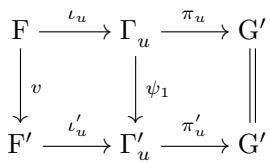
\includegraphics[keepaspectratio]{images/part002_ccea47d6.jpg}}

交换且 \(\varphi_{u}^{\prime}\circ\psi_{1}=\varphi_{v}\circ\varphi_{u}\)。\(\psi\) 的存在性由应用于 \(\psi_{1}\) 的命题 2 得出。反之，若 \(\psi^{\prime}\) 也具有所要的性质，则由引理 2 我们有 \(\psi^{\prime}\circ\varphi_{v}^{\prime}=\psi_{1}\)，故 \(\psi^{\prime}=\psi\)（命题 2）。

\subsection{\texorpdfstring{\(\tau\)-扩张的类上的群律}{\textbackslash tau-扩张的类上的群律}}

设 \(\mathrm{G}\) 是一个群，\(\mathrm{F}\) 是一个交换群，且 \(\tau : \mathrm{G} \to \mathrm{Aut}(\mathrm{F})\) 是一个群同态。用 \(\delta : \mathrm{G} \to \mathrm{G} \times \mathrm{G}\) 表示对角映射 \(g \mapsto (g, g)\)，并用 \(m : \mathrm{F} \times \mathrm{F} \to \mathrm{F}\) 表示乘法同态 \((f_1, f_2) \mapsto f_1 f_2\)。用 \(s : \mathrm{F} \to \mathrm{F}\) 表示由 \(f \mapsto f^{-1}\) 给出的群同态。设 \(\mathcal{E}_1 = (\Gamma_1, \iota_1, \pi_1)\) 与 \(\mathcal{E}_2 = (\Gamma_2, \iota_2, \pi_2)\) 是 \(\tau\)-扩张（\(\mathrm{G}\) 被 \(\mathrm{F}\) 的）。由于我们有关系

\[
m (((\tau \times \tau) \circ \delta) (g) \cdot (f _ {1}, f _ {2})) = \tau (g) \cdot m (f _ {1}, f _ {2})
\]

（对每个 \(g \in G\) 与所有 \(f_{1}, f_{2} \in F\)），扩张 \(m_{*}(\delta^{*}(\mathcal{E}_{1} \times \mathcal{E}_{2}))\) 是一个 \(\tau\)-扩张；我们称它为 \(\tau\)-扩张 \(E_{1}\) 与 \(E_{2}\) 的积，并记作 \(E_{1}E_{2}\)。这个扩张的类只依赖于扩张 \(E_{1}\) 与 \(E_{2}\) 的类（VIII, 第 288 页，推论 1 与 VIII, 第 291 页，推论 1）。于是这在 \(\operatorname{Ex}_{\tau}(\mathbf{G}, \mathbf{F})\) 上给出一个合成律。

注. —— 设 \(\mathcal{E}_{1}=(\Gamma_{1},\iota_{1},\pi_{1})\) 与 \(\mathcal{E}_{2}=(\Gamma_{2},\iota_{2},\pi_{2})\) 是 G 被 F 的 \(\tau\)-扩张。设 \(\mathcal{E}_{1}\mathcal{E}_{2}=(\Gamma,\iota,\pi)\) 是这些扩张的积。仿照 VIII, 第 289 页的例子，该构造给出一个从纤维积 \(\Gamma_{1}\times_{G}\Gamma_{2}\) 到 \(\Gamma\) 的满射群同态，其核是群同态 \(f\mapsto(\iota_{1}(f),\iota_{2}(f)^{-1})\)（从 F 到 \(\Gamma_{1}\times_{G}\Gamma_{2}\)）的像。

命题 4. —— \(\tau\)-扩张的积赋予集合 \(\mathrm{Ex}_{\tau}(\mathrm{G},\mathrm{F})\) 一个交换群的结构。它的单位元素是半平凡扩张 \(\mathcal{I}_{\tau}\) 的类。\(\tau\)-扩张 \(\mathcal{E}\) 的类的逆元是 \(s_{*}(\mathcal{E})\) 的类。

该律的结合性由诸图的交换性

\pandocbounded{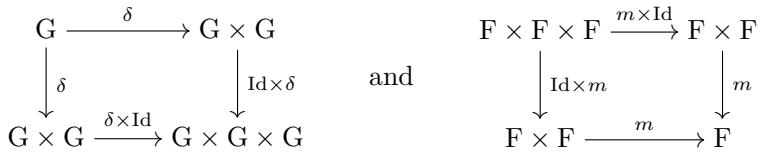
\includegraphics[keepaspectratio]{images/part002_39f17f00.jpg}}

以及 VIII, 第 288 页的推论 2、VIII, 第 291 页的推论 2 与 VIII, 第 292 页的命题 3 得出。

设 \(\Delta : \mathrm{F} \to \mathrm{F} \times \mathrm{F}\) 是对角映射 \(f \mapsto (f, f)\)。设 \(\mathcal{E} = (\Gamma, \iota, \pi)\) 是一个 \(\tau\)-扩张。设 \(\widetilde{\Delta}: \Gamma \to \Gamma \times_{\mathrm{G}} \Gamma\) 是由 \(\gamma \mapsto (\gamma, \gamma)\) 给出的群同态。下图交换：

\pandocbounded{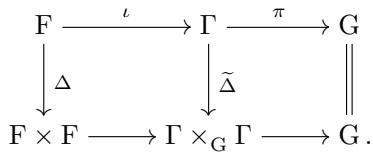
\includegraphics[keepaspectratio]{images/part002_db57599b.jpg}}

由 VIII, 第 290 页的命题 2 推出，\((\tau \times \tau) \circ \delta\)-扩张 \(\delta^{*}(\mathcal{E} \times \mathcal{E})\) 同构于 \(\Delta_{*}(\mathcal{E})\)。

用 \(c: F \to F\) 表示常值同态 \(f \mapsto 1\)。由 VIII, 第 292 页的例 1，\(\mathcal{I}_{\tau}\) 是这个合成律的单位元素这一事实由从 \(\delta^{*}(\mathcal{E} \times \mathcal{E})\) 到 \(\Delta_{*}(\mathcal{E})\) 的同构及交换图

\pandocbounded{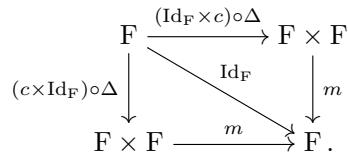
\includegraphics[keepaspectratio]{images/part002_761b87f2.jpg}}

最后一个断言由交换图

\[
\begin{array}{c} \mathrm{F} \xrightarrow {(\mathrm{Id} _ {\mathrm{F}} \times s) \circ \Delta} \mathrm{F} \times \mathrm{F} \\ (s \times \mathrm{Id} _ {\mathrm{F}}) \circ \Delta \Biggl \downarrow \qquad \qquad \qquad \qquad \qquad \qquad \qquad \qquad \qquad \qquad \qquad \qquad \qquad \qquad \qquad \qquad \qquad \qquad \qquad \qquad \qquad \qquad \qquad \qquad \qquad \qquad \qquad \qquad \qquad \qquad \qquad \qquad \qquad \qquad \\ \mathrm{F} \times \mathrm{F} \xrightarrow {m} \mathrm{F}. \end{array}
\]

设 \(\mathcal{E}_1 = (\Gamma_1,\iota_1,\pi_1)\) 与 \(\mathcal{E}_2 = (\Gamma_2,\iota_2,\pi_2)\) 是 \(\tau\)-扩张。群同构 \(\Gamma_1\times \Gamma_2\to \Gamma_2\times \Gamma_1\)（由 \((\gamma_{1},\gamma_{2})\mapsto (\gamma_{2},\gamma_{1})\) 给出）限制为群同构 \(\sigma :\Gamma_1\times_\mathrm{G}\Gamma_2\to \Gamma_2\times_\mathrm{G}\Gamma_1\)。由于关系

\[
\sigma (\iota_ {1} (f), \iota_ {2} (f) ^ {- 1}) = (\iota_ {2} (f ^ {- 1}), \iota_ {1} (f ^ {- 1}) ^ {- 1})
\]

（对 \(f \in F\)），群同态 \(\sigma\) 通过过渡到商诱导出一个 \(\tau\)-扩张的态射（从 \(E_{1}E_{2}\) 到 \(E_{2}E_{1}\) 的）。于是该合成律是交换的。

命题 5. —— a) 设 G 与 G' 是群，并设 F 是一个交换群。设 \(\tau: \mathrm{G} \to \operatorname{Aut}(\mathrm{F})\) 与 \(u: \mathrm{G}' \to \mathrm{G}\) 是群同态。映射 \(u^*: \operatorname{Ex}_{\tau}(\mathrm{G}, \mathrm{F}) \to \operatorname{Ex}_{\tau \circ u}(\mathrm{G}', \mathrm{F})\) 是一个群同态。

\begin{enumerate}
\def\labelenumi{\alph{enumi})}
\setcounter{enumi}{1}
\tightlist
\item
  设 G 是一个群，并设 F 与 \(F'\) 是交换群。设 \(\tau: G \to \text{Aut}(F)\)、\(\tau': G \to \text{Aut}(F')\) 与 \(v: F \to F'\) 是满足
\end{enumerate}

\[
\tau^ {\prime} (g) \cdot v (f) = v (\tau (g) \cdot f)
\]

（对 \(g \in \mathrm{G}\) 与 \(f \in \mathrm{F}\)）的群同态。映射 \(v_{*} : \operatorname{Ex}_{\tau}(\mathrm{G}, \mathrm{F}) \to \operatorname{Ex}_{\tau'}(\mathrm{G}, \mathrm{F}')\) 是一个群同态。

这由诸图的交换性得出

\[
\begin{array}{l} \mathrm{G} ^ {\prime} \xrightarrow {\delta} \mathrm{G} ^ {\prime} \times \mathrm{G} ^ {\prime} \\ \Biggl \downarrow_ {u} \qquad \Biggl \downarrow_ {u \times u} \\ \mathrm{G} \xrightarrow {\delta} \mathrm{G} \times \mathrm{G} \end{array} \qquad \text {and} \qquad \begin{array}{l} \mathrm{F} \times \mathrm{F} \xrightarrow {m} \mathrm{F} \\ \Biggl \downarrow_ {v \times v} \qquad \Biggl \downarrow_ {v} \\ \mathrm{F} ^ {\prime} \times \mathrm{F} ^ {\prime} \xrightarrow {m} \mathrm{F} ^ {\prime}. \end{array}
\]

\subsection{上同调描述}

设 G 是一个群，设 F 是一个交换群，并设 \(\tau: G \to \text{Aut}(F)\) 是一个群同态。对任何 \(g \in G\) 与 \(f \in F\)，我们也用 \(^{g}f\) 表示 \(\tau(g) \cdot f\)。G 的取值于 F 的一个 2-闭上链是指一个映射 \(c: G \times G \to F\)，使得对每个 \((g_{1}, g_{2}, g_{3}) \in G \times G \times G\)，我们有

\[
{ } ^ { g _ { 1 } } c ( g _ { 2 } , g _ { 3 } ) c ( g _ { 1 } , g _ { 2 } g _ { 3 } ) = c ( g _ { 1 } , g _ { 2 } ) c ( g _ { 1 } g _ { 2 } , g _ { 3 } ) .\tag{7}
\]

由于 F 是交换的，2-闭上链所成之集是从 \(G \times G\) 到 F 的映射所成的群的一个子群；我们把它记作 \(Z^{2}(G,F)\)。我们把从 G 到 F 的映射所成的群记作 \(C^{1}(G,F)\)。对每个 \(h \in C^{1}(G,F)\) 与 \((g_{1}, g_{2}) \in G \times G\)，令

\[
(\partial h) (g _ {1}, g _ {2}) = ^ {g _ {1}} h (g _ {2}) h (g _ {1} g _ {2}) ^ {- 1} h (g _ {1}).\tag{8}
\]

一个简单的计算表明映射 \(\partial h: G \times G \to F\) 是一个 2-闭上链。映射 \(\partial: C^{1}(G, F) \to Z^{2}(G, F)\) 是一个群同态。对任何 \(h \in C^{1}(G, F)\)，2-闭上链 \(\partial h\) 称为一个 2-上边缘。群

\(Z^{2}(G,F)/\partial(C^{1}(G,F))\) 记作 \(H^{2}(G,F)\)，称为以 F 为系数群的 G 的第二上同调群。

*上面的记号与 X, §6, n° 8, 第 112 页中关于群上同调的记号一致。*

设 \(\mathcal{E} = (\Gamma, \iota, \pi)\) 是一个 \(\tau\)-扩张。设 \(\sigma\) 是满射映射 \(\pi\) 的一个截面（集合论, II, §3, No.~8, 第 86 页），即一个从 G 到 \(\Gamma\) 的映射，使得 \(\pi(\sigma(g)) = g\)（对 G 中的每个 \(g\)）。对每对 \(g_1, g_2 \in G\)，\(\sigma(g_1)\sigma(g_2)\sigma(g_1g_2)^{-1}\) 属于 \(\mathrm{Ker}(\pi)\)，故存在唯一的映射 \(c_\sigma: G \times G \to F\)，使得

\[
\iota (c _ {\sigma} (g _ {1}, g _ {2})) = \sigma (g _ {1}) \sigma (g _ {2}) \sigma (g _ {1} g _ {2}) ^ {- 1}\tag{9}
\]

（对所有 \(g_{1}, g_{2} \in G\)）。映射 \(c_{\sigma}\) 是常值 1 的当且仅当 \(\sigma\) 是一个群同态。

命题 6. —— 映射 \(c_{\sigma}\) 是群 \(Z^{2}(G,F)\) 的一个元素，且它在上同调群 \(H^{2}(G,F)\) 中的类只依赖于 \(\tau\)-扩张 E 的类。

我们说映射 \(c_{\sigma}\) 是与 \(\sigma\) 相伴的 2-闭上链，而它在 \(\mathrm{H}^2 (\mathrm{G},\mathrm{F})\) 中的上同调类是 \(\tau\)-扩张 \(\mathcal{E}\) 的上同调类。

我们首先验证 \(c_{\sigma}\) 满足闭上链条件。设 \(g_{1}, g_{2}\) 与 \(g_{3}\) 是 G 的元素。利用 VIII, 第 285 页的公式 (1) 与 (9)，我们得到关系

\[
\begin{array}{r l} & {\iota (g _ {1} c _ {\sigma} (g _ {2}, g _ {3}) c _ {\sigma} (g _ {1}, g _ {2} g _ {3}))} \\ & {\quad = \sigma (g _ {1}) \sigma (g _ {2}) \sigma (g _ {3}) \sigma (g _ {2} g _ {3}) ^ {- 1} \sigma (g _ {1}) ^ {- 1} \sigma (g _ {1}) \sigma (g _ {2} g _ {3}) \sigma (g _ {1} g _ {2} g _ {3}) ^ {- 1}} \\ & {\quad = \sigma (g _ {1}) \sigma (g _ {2}) \sigma (g _ {3}) \sigma (g _ {1} g _ {2} g _ {3}) ^ {- 1}} \end{array}
\]

以及

\[
\begin{array}{r l} & {\iota (c _ {\sigma} (g _ {1}, g _ {2}) c _ {\sigma} (g _ {1} g _ {2}, g _ {3}))} \\ & {\qquad = \sigma (g _ {1}) \sigma (g _ {2}) \sigma (g _ {1} g _ {2}) ^ {- 1} \sigma (g _ {1} g _ {2}) \sigma (g _ {3}) \sigma (g _ {1} g _ {2} g _ {3}) ^ {- 1}} \\ & {\qquad = \sigma (g _ {1}) \sigma (g _ {2}) \sigma (g _ {3}) \sigma (g _ {1} g _ {2} g _ {3}) ^ {- 1}.} \end{array}
\]

于是映射 \(c_{\sigma}\) 是 \(\mathbf{Z}^2 (\mathrm{G},\mathrm{F})\) 的一个元素。

我们现在证明 \(c_{\sigma}\) 在 \(\mathrm{H}^{2}(\mathrm{G},\mathrm{F})\) 中的像不依赖于所选取的截面 \(\sigma\)。设 \(\sigma\) 与 \(\sigma'\) 是这样的截面。对 G 的每个元素 g，存在 F 的唯一元素 \(a_{g}\)，使得 \(\sigma'(g) = \iota(a_{g})\sigma(g)\)。设 \(g_{1}\) 与 \(g_{2}\) 是 G 的元素。利用定义 (9)，我们得到等式

\[
\begin{array}{r l} & {\iota (c _ {\sigma^ {\prime}} (g _ {1}, g _ {2})) = \sigma^ {\prime} (g _ {1}) \sigma^ {\prime} (g _ {2}) \sigma^ {\prime} (g _ {1} g _ {2}) ^ {- 1}} \\ & {\qquad = \iota (a _ {g _ {1}}) \sigma (g _ {1}) \iota (a _ {g _ {2}}) \sigma (g _ {2}) \sigma (g _ {1} g _ {2}) ^ {- 1} \iota (a _ {g _ {1} g _ {2}}) ^ {- 1}} \\ & {\qquad = \iota (a _ {g _ {1}}) \iota (^ {g _ {1}} a _ {g _ {2}}) \iota (c _ {\sigma} (g _ {1}, g _ {2})) \iota (a _ {g _ {1} g _ {2}}) ^ {- 1}.} \end{array}\tag{10}
\]

由于群 F 是交换的，我们有关系

\[
c _ {\sigma^ {\prime}} (g _ {1}, g _ {2}) c _ {\sigma} (g _ {1}, g _ {2}) ^ {- 1} = (^ {g _ {1}} a _ {g _ {2}}) a _ {g _ {1} g _ {2}} ^ {- 1} a _ {g _ {1}} = (\partial a) (g _ {1}, g _ {2}),\tag{11}
\]

这由 (8) 得出。这就证明了 \(c_{\sigma'}\) 与 \(c_{\sigma}\) 在 \(\mathrm{H}^2(\mathrm{G},\mathrm{F})\) 中的类重合。

最后，设 \(\mathcal{E} = (\Gamma, \iota, \pi)\) 与 \(\mathcal{E}' = (\Gamma', \iota', \pi')\) 是同构的 \(\tau\)-扩张，设 \(u: \mathcal{E} \to \mathcal{E}'\) 是一个 \(\tau\)-扩张的态射，并设 \(\sigma\) 是映射 \(\pi\) 的一个截面。映射 \(u \circ \sigma\) 是映射 \(\pi'\) 的一个截面，且我们有 \(c_{\sigma} = c_{u \circ \sigma}\)。于是 \(c_{\sigma}\) 在 \(\mathrm{H}^2(\mathrm{G}, \mathrm{F})\) 中的类只依赖于 \(\mathcal{E}\) 在 \(\mathrm{Ex}_{\tau}(\mathrm{G}, \mathrm{F})\) 中的类。

我们用 \(\Theta_{\tau}: \operatorname{Ex}_{\tau}(\mathrm{G},\mathrm{F}) \to \mathrm{H}^{2}(\mathrm{G},\mathrm{F})\)，或更简单地用 \(\Theta\)，表示把一个 \(\tau\)-扩张 \((\Gamma,\iota,\pi)\) 的类映到 2-闭上链 \(c_{\sigma}\) 的类的映射，其中 \(\sigma\) 是满射 \(\pi\) 的一个截面。

定理 1. —— 映射 \(\Theta\) 是从 \(\operatorname{Ex}_{\tau}(\mathrm{G},\mathrm{F})\) 到 \(\mathrm{H}^2 (\mathrm{G},\mathrm{F})\) 的一个群同构。

我们首先证明 \(\Theta\) 是一个群同态。设 \(\mathcal{E} = (\Gamma, \iota, \pi)\) 与 \(\mathcal{E}' = (\Gamma', \iota', \pi')\) 是 \(\tau\)-扩张，并设 \(\sigma\)（相应地，\(\sigma'\)）是映射 \(\pi\)（相应地，\(\pi'\)）的一个截面。我们用 \(\mathcal{E}\mathcal{E}' = (\Gamma'', \iota'', \pi'')\) 表示 \(\tau\)-扩张 E 与 \(E'\) 的积。我们用 \([\gamma, \gamma']\) 表示 \(\Gamma''\) 的元素，即元素 \((\gamma, \gamma')\)（\(\Gamma \times_{G} \Gamma'\) 中的）经 VIII, 第 293 页的注中的满射同态所得到的像。从 G 到 \(\Gamma''\) 的、把元素 g 映到 \([\sigma(g), \sigma'(g)]\) 的映射是一个截面 \(\sigma''\)（映射 \(\pi''\) 的）。设 \(g_1\) 与 \(g_2\) 是 G 的元素。我们有关系

\[
\begin{array}{r l} & {\iota^ {\prime \prime} (c _ {\sigma^ {\prime \prime}} (g _ {1}, g _ {2})) = \sigma^ {\prime \prime} (g _ {1}) \sigma^ {\prime \prime} (g _ {2}) \sigma^ {\prime \prime} (g _ {1} g _ {2}) ^ {- 1}} \\ & {\qquad = [ \iota (c _ {\sigma} (g _ {1}, g _ {2})), \iota^ {\prime} (c _ {\sigma^ {\prime}} (g _ {1}, g _ {2}) ]} \\ & {\qquad = \iota^ {\prime \prime} (c _ {\sigma} (g _ {1}, g _ {2}) c _ {\sigma^ {\prime}} (g _ {1}, g _ {2})).} \end{array}
\]

于是我们有 \(c_{\sigma''}(g_1, g_2) = c_\sigma(g_1, g_2)c_{\sigma'}(g_1, g_2)\)。

我们证明映射 \(\Theta\) 是单射。设 \(\mathcal{E} = (\Gamma, \iota, \pi)\) 是一个 \(\tau\)-扩张，并设 \(\sigma\) 是映射 \(\pi\) 的一个截面，使得 \(c_{\sigma}\) 在 \(\mathrm{H}^{2}(\mathrm{G}, \mathrm{F})\) 中的像是平凡的。存在一个映射 \(a : G \to F\)，使得

\[
c _ {\sigma} (g _ {1}, g _ {2}) = (^ {g _ {1}} a (g _ {2})) a (g _ {1} g _ {2}) ^ {- 1} a (g _ {1})
\]

对所有 \(g_{1}, g_{2} \in G\)。然后我们用下式定义 \(\sigma' : G \to \Gamma\)

\[
\sigma^ {\prime} (g) = \iota (a (g) ^ {- 1}) \sigma (g)
\]

对 \(g \in G\)。利用 (11)，我们得到 \(c_{\sigma'}\) 是取常值 1 的映射；于是 \(\sigma'\) 是一个群同态，这就证明了 \(\tau\)-扩张 E 是半平凡的（I, §6, No.~1, 第 67 页, 命题 4）。

我们证明映射 \(\Theta\) 是满射。设 c 是 \(Z^{2}(G,F)\) 的一个元素。我们给集合 \(\Gamma = F \times G\) 赋以如下的合成律：

\[
(f _ {1}, g _ {1}) (f _ {2}, g _ {2}) = \left(f _ {1} (^ {g _ {1}} f _ {2}) c (g _ {1}, g _ {2}), g _ {1} g _ {2}\right)\tag{12}
\]

对所有 \(f_{1}, f_{2} \in F\) 与 \(g_{1}, g_{2} \in G\)。我们有关系

\[
\begin{array}{r l} (f _ {1}, g _ {1}) ((f _ {2}, g _ {2}) (f _ {3}, g _ {3})) & = (f _ {1}, g _ {1}) \big (f _ {2} (^ {g _ {2}} f _ {3}) c (g _ {2}, g _ {3}), g _ {2} g _ {3} \big) \\ & = \big (f _ {1} (^ {g _ {1}} f _ {2}) (^ {g _ {1} g _ {2}} f _ {3}) (^ {g _ {1}} c (g _ {2}, g _ {3})) c (g _ {1}, g _ {2} g _ {3}), g _ {1} g _ {2} g _ {3} \big) \end{array}
\]

以及

\[
\begin{array}{c} ((f _ {1}, g _ {1}) (f _ {2}, g _ {2}))   (f _ {3}, g _ {3}) = \big (f _ {1} (^ {g _ {1}} f _ {2}) c (g _ {1}, g _ {2}), g _ {1} g _ {2} \big) (f _ {3}, g _ {3}) \\ = \big (f _ {1} (^ {g _ {1}} f _ {2}) (^ {g _ {1} g _ {2}} f _ {3}) c (g _ {1}, g _ {2}) c (g _ {1} g _ {2}, g _ {3}), g _ {1} g _ {2} g _ {3} \big) \end{array}
\]

对所有 \(f_{1}, f_{2}, f_{3} \in F\) 与 \(g_{1}, g_{2}, g_{3} \in G\)。由此推出该律是结合的，因为 c 是一个 2-闭上链。对每个 \((f, g) \in \Gamma\)，我们有

\[
(f, g) (c (e, e) ^ {- 1}, e) = (f (^ {g} c (e, e) ^ {- 1}) c (g, e), g).
\]

另一方面，由 2-闭上链的定义推出 \(c(g, e) = {}^g c(e, e)\)，由此我们推出 \((f, g)(c(e, e)^{-1}, e) = (f, g)\)。我们同理证明

\[
(c (e, e) ^ {- 1}, e) (f, g) = (f c (e, e) ^ {- 1} c (e, g), g) = (f, g).
\]

于是由 (12) 定义的合成律有单位元素 \((c(e,e)^{-1},e)\)，且每个元素 \((f,g)\)（属于 \(\Gamma\)）都是可逆的，其逆为

\[
\left(^ {g ^ {- 1}} (f ^ {- 1} c (e, e) ^ {- 1} c (g, g ^ {- 1}) ^ {- 1}), g ^ {- 1}\right).
\]

这样我们就给 \(\Gamma\) 装备了一个群结构。我们用 \(\iota: F \to G\) 表示把 f 映到 \((c(e, e)^{-1}f, e)\) 的映射，用 \(\pi: \Gamma \to G\) 表示第二个投影，并用 \(\sigma\) 表示映射 \(g \mapsto (1, g)\)。映射 \(\iota\) 与 \(\pi\) 是群同态，于是三元组 \(\mathcal{E} = (\Gamma, \iota, \pi)\) 是一个 \(\tau\)-扩张，\(\sigma\) 是映射 \(\pi\) 的一个截面，并且相伴的闭上链 \(c_{\sigma}\) 等于 c，因为

\[
\begin{array}{c} \sigma (g _ {1}) \sigma (g _ {2}) \sigma (g _ {1} g _ {2}) ^ {- 1} = (1, g _ {1}) (1, g _ {2}) (1, g _ {1} g _ {2}) ^ {- 1} = (c (g _ {1}, g _ {2}), g _ {1} g _ {2}) (1, g _ {1} g _ {2}) ^ {- 1} \\ = (c (g _ {1}, g _ {2}) c (e, g _ {1} g _ {2}) ^ {- 1}, e) = (c (e, e) ^ {- 1} c (g _ {1}, g _ {2}), e) \end{array}
\]

对 \(g_{1}, g_{2} \in G\)。

注. —— 设 G 是一个群，设 F 与 \(F'\) 是交换群， 设 \(\tau\)（相应地，\(\tau'\)）是从 G 到 F（相应地，\(F'\)）的自同构群的一个群同态，并设 \(v : F \to F'\) 是一个群态射，使得

\[
v (\tau (g) \cdot f) = \tau^ {\prime} (g) \cdot v (f)\tag{13}
\]

对 \(g \in G\) 与 \(f \in F\)。设 \(\alpha\) 是 \(\operatorname{Ex}_{\tau}(\mathrm{G}, \mathrm{F})\) 的一个元素。若闭上链 c 代表 \(\Theta(\alpha)\)，则 \(v \circ c\) 代表 \(\Theta(v_{*}(\alpha)) \in \mathrm{H}^{2}(\mathrm{G}, \mathrm{F}')\)。

\subsection{限制与余限制}

设 G 与 \(G'\) 是群，F 是交换群，而 \(\tau\) 是从 G 到 F 的自同构群的一个同态。设 \(u: G' \to G\) 是一个群同态。我们记 \(\tau' = \tau \circ u\)。

若 \(\psi : \mathrm{G} \times \mathrm{G} \to \mathrm{F}\) 是 \(\mathrm{G}\) 的取值于 \(\mathrm{F}\) 的一个 2-闭上链，则映射 \(\psi \circ (u \times u)\)（从 \(\mathrm{G}' \times \mathrm{G}'\) 到 \(\mathrm{F}\)，由 \((g_1, g_2) \mapsto \psi(u(g_1), u(g_2))\) 给出）是 \(\mathrm{G}'\) 的取值于 \(\mathrm{F}\) 的一个 2-闭上链，且映射 \(\psi \mapsto \psi \circ (u \times u)\)（从 \(\mathrm{Z}^2(\mathrm{G}, \mathrm{F})\) 到 \(\mathrm{Z}^2(\mathrm{G}', \mathrm{F})\)）诱导一个群同态 \(u^*: \mathrm{H}^2(\mathrm{G}, \mathrm{F}) \to \mathrm{H}^2(\mathrm{G}', \mathrm{F})\)。对任何 \(\lambda \in \mathrm{H}^2(\mathrm{G}, \mathrm{F})\)，元素 \(u^*(\lambda)\) 称为 \(\lambda\) 被 \(u\) 的逆像。当 \(\mathrm{G}'\) 是 \(\mathrm{G}\) 的子群且 \(u: \mathrm{G}' \to \mathrm{G}\) 是典范单射时，同态 \(u^*\) 称为从 \(\mathrm{G}\) 到 \(\mathrm{G}'\) 的限制同态；我们把它记作 \(\operatorname{Res}_{\mathrm{G}'}^{\mathrm{G}}\)。当 \(\mathrm{G}\) 是 \(\mathrm{G}'\) 的商且 \(u: \mathrm{G}' \to \mathrm{G}\) 是典范满射时，同态 \(u^*\) 称为从 \(\mathrm{G}\) 到 \(\mathrm{G}'\) 的膨胀同态。

命题 7. —— 用上面的记号，下图交换：

\[
\begin{array}{c} \operatorname{Ex} _ {\tau} (\mathrm{G}, \mathrm{F}) \xrightarrow {u ^ {*}} \operatorname{Ex} _ {\tau} (\mathrm{G} ^ {\prime}, \mathrm{F}) \\ \Biggl \downarrow \Theta_ {\tau} \qquad \qquad \qquad \Biggl \downarrow \Theta_ {\tau^ {\prime}} \\ \operatorname{H} ^ {2} (\mathrm{G}, \mathrm{F}) \xrightarrow {u ^ {*}} \operatorname{H} ^ {2} (\mathrm{G} ^ {\prime}, \mathrm{F})  . \end{array}
\]

设 H 是 G 的一个有限指数子群。设 s 是从 G 到 \(H\backslash G\) 的典范满射的一个截面。我们用 \((g,x)\mapsto x\cdot g\) 表示由 G 借乘法在其自身上的右作用所诱导的 G 在 \(H\backslash G\) 上的右作用。注意对每个 \(x\in H\backslash G\) 与 \(g\in G\)，元素 \(s(x)gs(x\cdot g)^{-1}\) 属于 H。于是对任何映射 \(c: \mathrm{H} \times \mathrm{H} \to \mathrm{F}\)，我们都可以用关系式定义一个映射 \(\widetilde{c}_s: \mathrm{G} \times \mathrm{G} \to \mathrm{F}\)

\[
\widetilde {c} _ {s} (g _ {1}, g _ {2}) = \prod_ {x \in \mathrm{H} \backslash \mathrm{G}} ^ {s (x) ^ {- 1}} c \bigl (s (x) g _ {1} s (x \cdot g _ {1}) ^ {- 1}, s (x \cdot g _ {1}) g _ {2} s (x \cdot g _ {1} g _ {2}) ^ {- 1} \bigr)
\]

对 \(g_{1}, g_{2} \in G\)。映射 \(c \mapsto \widetilde{c}_{s}\) 是从 \(F^{H \times H}\) 到 \(F^{G \times G}\) 的一个群同态。

引理 4. —— 若 \(c: \mathrm{H} \times \mathrm{H} \to \mathrm{F}\) 是 H 的取值于 F 的一个 2-闭上链，则 \(\widetilde{c}_s\) 是 G 的取值于 F 的一个 2-闭上链。

设 \(g_1, g_2\) 与 \(g_3\) 是 G 的元素。对每个 \(i \in \{1, 2, 3\}\)，我们用关系式定义一个映射 \(h_i: \mathrm{H} \backslash \mathrm{G} \to \mathrm{H}\)

\[
h _ {i} (x) = s \left(x \cdot g _ {1} \dots g _ {i - 1}\right) g _ {i} s \left(x \cdot g _ {1} \dots g _ {i}\right) ^ {- 1}
\]

对 \(x\in \mathrm{H}\backslash \mathrm{G}\)。注意

\[
\begin{array}{l} {h _ {1} (x) h _ {2} (x) = s (x) g _ {1} g _ {2} s (x \cdot g _ {1} g _ {2}) ^ {- 1}} \\ {h _ {2} (x) h _ {3} (x) = s (x \cdot g _ {1}) g _ {2} g _ {3} s (x \cdot g _ {1} g _ {2} g _ {3}) ^ {- 1}} \end{array}
\]

对 \(x \in \mathrm{H} \backslash \mathrm{G}\)。于是我们有关系

\[
\begin{array}{r l} & ^ {g _ {1}} \widetilde {c} _ {s} (g _ {2}, g _ {3}) \widetilde {c} _ {s} (g _ {1} g _ {2}, g _ {3}) ^ {- 1} \widetilde {c} _ {s} (g _ {1}, g _ {2} g _ {3}) \widetilde {c} _ {s} (g _ {1}, g _ {2}) ^ {- 1} \\ & \quad = \prod_ {x \in \mathrm{H} \backslash \mathrm{G}} ^ {g _ {1} s (x) ^ {- 1}} c \big (s (x) g _ {2} s (x \cdot g _ {2}) ^ {- 1}, s (x \cdot g _ {2}) g _ {3} s (x \cdot g _ {2} g _ {3}) ^ {- 1} \big) \\ & \qquad \times \prod_ {x \in \mathrm{H} \backslash \mathrm{G}} ^ {s (x) ^ {- 1}} \Big (c (h _ {1} (x) h _ {2} (x), h _ {3} (x)) ^ {- 1} \\ & \qquad \qquad \qquad \qquad \times c (h _ {1} (x), h _ {2} (x) h _ {3} (x))   c (h _ {1} (x), h _ {2} (x)) ^ {- 1} \Big) \\ & = \prod_ {x \in \mathrm{H} \backslash \mathrm{G}} ^ {s (x \cdot g _ {1} ^ {- 1}) ^ {- 1} h _ {1} (x \cdot g _ {1} ^ {- 1})} c (h _ {2} (x \cdot g _ {1} ^ {- 1}), h _ {3} (x \cdot g _ {1} ^ {- 1})) \\ & \qquad \times \prod_ {x \in \mathrm{H} \backslash \mathrm{G}} ^ {s (x) ^ {- 1} h _ {1} (x)} c (h _ {2} (x), h _ {3} (x)) ^ {- 1} \\ & = 1, \end{array}
\]

其中第二个等式由 c 是 2-闭上链这一事实得出。

引理 5. —— 若 \(c\) 是一个 2-上边缘，则 \(\widetilde{c}_s\) 也是。

设 \(t: \mathrm{H} \to \mathrm{F}\) 是使得 \(c = \partial t\) 的一个映射。设 \(\widetilde{t}_s: \mathrm{G} \to \mathrm{F}\) 是由下式定义的映射

\[
\widetilde {t} _ {s} (g) = \prod_ {x \in \mathrm{H} \backslash \mathrm{G}} ^ {s (x) ^ {- 1}} t (s (x) g s (x \cdot g) ^ {- 1})
\]

对 \(g \in G\)。只需证明 \(\widetilde{c}_{s} = \partial\widetilde{t}_{s}\)，这由关系

\[
\begin{array}{l} \widetilde {c} _ {s} (g _ {1}, g _ {2}) = \prod_ {x \in \mathrm{H} \backslash \mathrm{G}} ^ {s (x) ^ {- 1} s (x) g _ {1} s (x \cdot g _ {1}) ^ {- 1}} t (s (x \cdot g _ {1}) g _ {2} s (x \cdot g _ {1} g _ {2}) ^ {- 1}) \\ \qquad \times \prod_ {x \in \mathrm{H} \backslash \mathrm{G}} ^ {s (x) ^ {- 1}} \big (t (s (x) g _ {1} g _ {2} s (x \cdot g _ {1} g _ {2}) ^ {- 1}) ^ {- 1} t (s (x) g _ {1} s (x \cdot g _ {1}) ^ {- 1}) \big) \\ = \partial \widetilde {t} _ {s} (g _ {1}, g _ {2}) \end{array}
\]

对 \(g_{1}, g_{2} \in G\) 得出。

引理 6. —— 设 c 是 H 的取值于 F 的一个 2-闭上链。\(\widetilde{c}_{s}\) 在群 \(\mathrm{H}^{2}(\mathrm{G},\mathrm{F})\) 中的像不依赖于截面 s 的选取。

设 \(s'\) 是从 G 到 \(H\backslash G\) 的典范满射的一个截面。设 \(h: \mathrm{H} \backslash \mathrm{G} \to \mathrm{H}\) 是由关系式

\[
s ^ {\prime} (x) = h (x) s (x)
\]

对 \(x \in H \backslash G\) 刻画的映射。于是 2-闭上链 \(\widetilde{c}_{s'}\) 由关系式给出

\[
\begin{array}{l} \widetilde {c} _ {s ^ {\prime}} (g _ {1}, g _ {2}) \\ = \prod_ {x \in \mathrm{H} \backslash \mathrm{G}} ^ {s (x) ^ {- 1} h (x) ^ {- 1}} c \big (h (x) s (x) g _ {1} s ^ {\prime} (x \cdot g _ {1}) ^ {- 1}, s ^ {\prime} (x \cdot g _ {1}) g _ {2} s ^ {\prime} (x \cdot g _ {1} g _ {2}) ^ {- 1} \big) \\ = \prod_ {x \in \mathrm{H} \backslash \mathrm{G}} ^ {s (x) ^ {- 1}} c \big (s (x) g _ {1} s (x \cdot g _ {1}) ^ {- 1} h (x \cdot g _ {1}) ^ {- 1}, h (x \cdot g _ {1}) s (x \cdot g _ {1}) g _ {2} s ^ {\prime} (x \cdot g _ {1} g _ {2}) ^ {- 1} \big) \\ \qquad \times \prod_ {x \in \mathrm{H} \backslash \mathrm{G}} ^ {s (x) ^ {- 1}} \Big (c \big (h (x) ^ {- 1}, s ^ {\prime} (x) g _ {1} g _ {2} s ^ {\prime} (x \cdot g _ {1} g _ {2}) ^ {- 1} \big) ^ {- 1} \\ \qquad \qquad \qquad \qquad \qquad \qquad \qquad \qquad \qquad \qquad \qquad \qquad \qquad \qquad \qquad \qquad \qquad \qquad \qquad \qquad \qquad \qquad \qquad \qquad \qquad \qquad \qquad \qquad \qquad \qquad \qquad \qquad \qquad \qquad \\ = \prod_ {x \in \mathrm{H} \backslash \mathrm{G}} ^ {g _ {1} s (x \cdot g _ {1}) ^ {- 1}} c \big (h (x \cdot g _ {1}) ^ {- 1}, h (x \cdot g _ {1}) s (x \cdot g _ {1}) g _ {2} s ^ {\prime} (x \cdot g _ {1} g _ {2}) ^ {- 1} \big) \\ \qquad \times \prod_ {x \in \mathrm{H} \backslash \mathrm{G}} ^ {s (x) ^ - 1} c \big (s (x) g _ {1} s (x \cdot g _ {1}) ^ {- 1}, s (x \cdot g _ {1}) g _ {2} s ^ {\prime} (x \cdot g _ {1} g _ {2}) ^ {- 1} \big) \\ \qquad \times \prod_ {x \in \mathrm{H} \backslash \mathrm{G}} ^ {s (x) ^ {- 1}} c \big (s (x) g _ {1} s (x \cdot g _ {1}) ^ {- 1}, h (x \cdot g _ {1}) ^ {- 1} \big) ^ {- 1} \\ \qquad \times \prod_ {x \in \mathrm{H} \backslash \mathrm{G}} ^ {s (x) ^ {- 1}} \Big (c \big (h (x) ^ {- 1}, s ^ {\prime} (x) g _ {1} g _ {2} s ^ {\prime} (x \cdot g _ {1} g _ {2}) ^ {- 1} \big) ^ {{- 1}} \\ \qquad \qquad \qquad \qquad \qquad \qquad \qquad \qquad \qquad \qquad \qquad \qquad \times c (h (x) ^ {- 1}, s ^ {\prime} (x) g _ {1} s ^ {\prime} (x \cdot g _ {1}) ^ {- 1})   {\Big)} \end{array}
\]

\[
\begin{array}{l} = \prod_ {x \in \mathrm{H} \backslash \mathrm{G}} ^ {s (x) ^ {- 1}} c \big (s (x) g _ {1} s (x \cdot g _ {1}) ^ {- 1}, s (x \cdot g _ {1}) g _ {2} s ^ {\prime} (x \cdot g _ {1} g _ {2}) ^ {- 1} \big) \\ \qquad \times \prod_ {x \in \mathrm{H} \backslash \mathrm{G}} ^ {s (x) ^ {- 1}} c \big (s (x) g _ {1} s (x \cdot g _ {1}) ^ {- 1}, h (x \cdot g _ {1}) ^ {- 1} \big) ^ {- 1} \\ \qquad \times \prod_ {x \in \mathrm{H} \backslash \mathrm{G}} ^ {g _ {1} s (x) ^ {- 1}} c \big (h (x) ^ {- 1}, h (x) s (x) g _ {2} s ^ {\prime} (x \cdot g _ {2}) ^ {- 1} \big) \\ \qquad \times \prod_ {x \in \mathrm{H} \backslash \mathrm{G}} ^ {s (x) ^ {- 1}} \Big (c \big (h (x) ^ {- 1}, s ^ {\prime} (x) g _ {1} g _ {2} s ^ {\prime} (x \cdot g _ {1} g _ {2}) ^ {- 1} \big) ^ {- 1} \\ \qquad \qquad \qquad \qquad \qquad \qquad \qquad \qquad \qquad \qquad \qquad \qquad \qquad \qquad \qquad \qquad \qquad \qquad \times c \big (h (x) ^ {- 1}, s ^ {\prime} (x) g _ {1} s ^ {\prime} (x \cdot g _ {1}) ^ {- 1} \big) \Big) \end{array}
\]

对所有 \(g_1, g_2 \in \mathbf{G}\)。第一个等式来自把闭上链关系（VIII, 第 295 页, 公式 (7)）应用于元素

\[
h (x) ^ {- 1}, \quad h (x) s (x) g _ {1} s ^ {\prime} (x \cdot g _ {1}) ^ {- 1}, \quad \mathrm{and} \quad s ^ {\prime} (x \cdot g _ {1}) g _ {2} s ^ {\prime} (x \cdot g _ {1} g _ {2}) ^ {- 1};
\]

第二个等式是通过对元素

\[
s (x) g _ {1} s \left(x \cdot g _ {1}\right) ^ {- 1}, \quad h \left(x \cdot g _ {1}\right) ^ {- 1}, \quad \text { and } \quad h \left(x \cdot g _ {1}\right) s \left(x \cdot g _ {1}\right) g _ {2} s ^ {\prime} \left(x \cdot g _ {1} g _ {2}\right) ^ {- 1};
\]

而最后一个等式只是用到了映射 \(x \mapsto x \cdot g_{1}\) 是 \(H\backslash G\) 的一个置换这一事实。

所得表达式的最后两行对应于一个 2-上边缘。我们发现 \(\widetilde{c}_{s'}\) 在 \(\mathrm{H}^2 (\mathrm{G},\mathrm{F})\) 中与那个在 \((g_{1},g_{2})\in \mathrm{G}^{2}\) 处的值由下述表达式给出的闭上链有相同的类

\[
\begin{array}{l} \prod_ {x \in \mathrm{H} \backslash \mathrm{G}} ^ {s (x) ^ {- 1}} c \big (s (x) g _ {1} s (x \cdot g _ {1}) ^ {- 1}, s (x \cdot g _ {1}) g _ {2} s (x \cdot g _ {1} g _ {2}) ^ {- 1} h (x \cdot g _ {1} g _ {2}) ^ {- 1} \big) \\ \qquad \qquad \qquad \times \prod_ {x \in \mathrm{H} \backslash \mathrm{G}} ^ {s (x) ^ {- 1}} c \big (s (x) g _ {1} s (x \cdot g _ {1}) ^ {- 1}, h (x \cdot g _ {1}) ^ {- 1} \big) ^ {- 1} \\ = \prod_ {x \in \mathrm{H} \backslash \mathrm{G}} ^ {g _ {1} s (x \cdot g _ {1}) ^ {- 1}} c \big (s (x \cdot g _ {1}) g _ {2} s (x \cdot g _ {1} g _ {2}) ^ {- 1}, h (x \cdot g _ {1} g _ {2}) ^ {- 1} \big) ^ {- 1} \\ \qquad \qquad \times \prod_ {x \in \mathrm{H} \backslash \mathrm{G}} ^ {s (x) ^ {- 1}} c \big (s (x) g _ {1} s (x \cdot g _ {1}) ^ {- 1}, s (x \cdot g _ {1}) g _ {2} s (x \cdot g _ {1} g _ {2}) ^ {- 1} \big) \\ \qquad \qquad \times \prod_ {x \in \mathrm{H} \backslash \mathrm{G}} ^ {s (x) ^ {- 1}} \Big (c \big (s (x) g _ {1} g _ {2} s (x \cdot g _ {1} g _ {2}) ^ {- 1}, h (x \cdot g _ {1} g _ {2}) ^ {- 1} \big) \\ \qquad \qquad \qquad \times c \big (s (x) g _ {1} s (x \cdot g _ {1}) ^ {- 1}, h (x \cdot g _ {1}) ^ {- 1} \big) ^ {- 1} \Big) \end{array}
\]

\[
\begin{array}{l} = \prod_ {x \in \mathrm{H} \backslash \mathrm{G}} ^ {s (x) ^ {- 1}} c \big (s (x) g _ {1} s (x \cdot g _ {1}) ^ {- 1}, s (x \cdot g _ {1}) g _ {2} s (x \cdot g _ {1} g _ {2}) ^ {- 1} \big) \\ \quad \times \prod_ {x \in \mathrm{H} \backslash \mathrm{G}} ^ {g _ {1} s (x) ^ {- 1}} c \big (s (x) g _ {2} s (x \cdot g _ {2}) ^ {- 1}, h (x \cdot g _ {2}) ^ {- 1} \big) ^ {- 1} \\ \quad \times \prod_ {x \in \mathrm{H} \backslash \mathrm{G}} ^ {s (x) ^ {- 1}} \Big (c \big (s (x) g _ {1} g _ {2} s (x \cdot g _ {1} g _ {2}) ^ {- 1}, h (x \cdot g _ {1} g _ {2}) ^ {- 1} \big) \\ \qquad \qquad \qquad \qquad \qquad \qquad \qquad \qquad \qquad \qquad \qquad \qquad \qquad \times c \big (s (x) g _ {1} s (x \cdot g _ {1}) ^ {- 1}, h (x \cdot g _ {1}) ^ {- 1} \big) ^ {- 1} \Big), \end{array}
\]

其中第一个等式由对元素应用闭上链关系得出

\[
s (x) g _ {1} s (x \cdot g _ {1}) ^ {- 1}, \quad s (x \cdot g _ {1}) g _ {2} s (x \cdot g _ {1} g _ {2}) ^ {- 1}, \quad \text { and } \quad h (x \cdot g _ {1} g _ {2}) ^ {- 1}.
\]

所得表达式的最后两行对应于一个 2-上边缘。我们发现 \(\widetilde{c}_{s'}\) 的类与 \(\widetilde{c}_s\) 的类重合。

我们已经构造了一个从群 \(\mathrm{H}^{2}(\mathrm{H},\mathrm{F})\) 到群 \(\mathrm{H}^{2}(\mathrm{G},\mathrm{F})\) 的同态，我们称它为从 H 到 G 的余限制同态，并记作 \(Cor_{H}^{G}\)。

命题 8. —— 设 H 是 G 的一个有限指数子群。自同态 \(Cor_{H}^{G} \circ Res_{H}^{G}\)（群 \(H^{2}(G, F)\) 的）与用指数 \((G : H)\) 作乘法相重合。

设 \(\alpha\) 是 \(\mathrm{H}^2 (\mathrm{G},\mathrm{F})\) 的一个元素，并设 \(c\) 是 \(\mathrm{Z}^2 (\mathrm{G},\mathrm{F})\) 的一个元素，它代表 \(\alpha\)。元素 \(\mathrm{Cor}_{\mathrm{H}}^{\mathrm{G}}\circ \mathrm{Res}_{\mathrm{H}}^{\mathrm{G}}(\alpha)\) 是那个在 \((g_{1},g_{2})\in \mathrm{G}^{2}\) 处的值由下述表达式给出的闭上链的类

\[
\begin{array}{l} \prod_ {x \in \mathrm{H} \backslash \mathrm{G}} ^ {s (x) ^ {- 1}} c (s (x) g _ {1} s (x \cdot g _ {1}) ^ {- 1}, s (x \cdot g _ {1}) g _ {2} s (x \cdot g _ {1} g _ {2}) ^ {- 1}) \\ = \prod_ {x \in \mathrm{H} \backslash \mathrm{G}} c (g _ {1} s (x \cdot g _ {1}) ^ {- 1}, s (x \cdot g _ {1}) g _ {2} s (x \cdot g _ {1} g _ {2}) ^ {- 1}) \\ \quad \times \prod_ {x \in \mathrm{H} \backslash \mathrm{G}} \big (c (s (x) ^ {- 1}, s (x) g _ {1} g _ {2} s (x \cdot g _ {1} g _ {2}) ^ {- 1}) ^ {- 1} c (s (x) ^ {- 1}, s (x) g _ {1} s (x \cdot g _ {1}) ^ {- 1}) \big) \\ = \prod_ {x \in \mathrm{H} \backslash \mathrm{G}} ^ {g _ {1}} c (s (x \cdot g _ {1}) ^ {- 1}, s (x \cdot g _ {1}) g _ {2} s (x \cdot g _ {1} g _ {2}) ^ {- 1}) \\ \quad \times \prod_ {x \in \mathrm{H} \backslash \mathrm{G}} c (g _ {1}, g _ {2} s (x \cdot g _ {1} g _ {2}) ^ {- 1}) c (g _ {1}, s (x \cdot g _ {1}) ^ {- 1}) ^ {- 1} \\ \quad \times \prod_ {x \in \mathrm{H} \backslash \mathrm{G}} \big (c (s (x) ^ {- 1}, s (x) g _ {1} g _ {2} s (x \cdot g _ {1} g _ {2}) ^ {- 1}) ^ {- 1} c (s (x) ^ {- 1}, s (x) g _ {1} s (x \cdot g _ {1}) ^ {- 1}) \big) \end{array}
\]

\[
\begin{array}{l} = \prod_ {x \in \mathrm{H} \backslash \mathrm{G}} c (g _ {1}, g _ {2} s (x \cdot g _ {1} g _ {2}) ^ {- 1}) c (g _ {1}, s (x \cdot g _ {1}) ^ {- 1}) ^ {- 1} \\ \times \prod_ {x \in \mathrm{H} \backslash \mathrm{G}} ^ {g _ {1}} c (s (x) ^ {- 1}, s (x) g _ {2} s (x g _ {2}) ^ {- 1}) \\ \times \prod_ {x \in \mathrm{H} \backslash \mathrm{G}} \left(c (s (x) ^ {- 1}, s (x) g _ {1} g _ {2} s (x \cdot g _ {1} g _ {2}) ^ {- 1}) ^ {- 1} c (s (x) ^ {- 1}, s (x) g _ {1} s (x \cdot g _ {1}) ^ {- 1})\right). \end{array}
\]

第一个等式来自把闭上链关系（VIII, 第 295 页, 公式 (7)）应用于元素

\[
s (x) ^ {- 1}, \quad s (x) g _ {1} s (x \cdot g _ {1}) ^ {- 1}, \quad \mathrm{and} \quad s (x \cdot g _ {1}) g _ {2} s (x \cdot g _ {1} g _ {2}) ^ {- 1};
\]

第二个等式是通过对元素

\[
g _ {1}, \quad s (x \cdot g _ {1}) ^ {- 1}, \quad \mathrm{and} \quad s (x \cdot g _ {1}) g _ {2} s (x \cdot g _ {1} g _ {2}) ^ {- 1}.
\]

通过去掉一个上边缘，我们得到 \(\mathrm{Cor}_{\mathrm{H}}^{\mathrm{G}} \circ \mathrm{Res}_{\mathrm{H}}^{\mathrm{G}}(\alpha)\) 是那个在 \((g_{1}, g_{2}) \in \mathrm{G}^{2}\) 处的值由下述表达式给出的闭上链的类

\[
\begin{array}{l} \prod_ {x \in \mathrm{H} \backslash \mathrm{G}} c (g _ {1}, g _ {2} s (x \cdot g _ {1} g _ {2}) ^ {- 1}) c (g _ {1}, s (x \cdot g _ {1}) ^ {- 1}) ^ {- 1} \\ = \prod_ {x \in \mathrm{H} \backslash \mathrm{G}} ^ {g _ {1}} c (g _ {2}, s (x \cdot g _ {1} g _ {2}) ^ {- 1}) ^ {- 1} c (g _ {1} g _ {2}, s (x \cdot g _ {1} g _ {2}) ^ {- 1}) c (g _ {1}, g _ {2}) \\ \times \prod_ {x \in \mathrm{H} \backslash \mathrm{G}} c (g _ {1}, s (x \cdot g _ {1}) ^ {- 1}) ^ {- 1} \\ = \prod_ {x \in \mathrm{H} \backslash \mathrm{G}} ^ {g _ {1}} c (g _ {2}, s (x \cdot g _ {2}) ^ {- 1}) ^ {- 1} c (g _ {1} g _ {2}, s (x \cdot g _ {1} g _ {2}) ^ {- 1}) c (g _ {1}, s (x \cdot g _ {1}) ^ {- 1}) ^ {- 1} \\ \times c (g _ {1}, g _ {2}) ^ {\text {(G:H)}}, \end{array}
\]

这就证明了结论。

\subsection{伽罗瓦代数}

设 K 是一个交换域。若 E 是一个 K-代数，则我们用 \(\operatorname{Aut}_{\mathrm{K}}(\mathrm{E})\) 表示它的自同构群。若 E 是体 K 的一个伽罗瓦扩张，则群 \(\operatorname{Aut}_{\mathrm{K}}(\mathrm{E})\) 就是伽罗瓦群 \(\operatorname{Gal}(\mathrm{E}/\mathrm{K})\)（V, §10, No.~2, 第 58 页）。

设 G 是一个群。一个 \((K,G)\)-代数是装备了一个群同态 \(\lambda:G\to\operatorname{Aut}_{K}(E)\) 的 K-代数 E。于是同态 \(\lambda\) 给 E 装备了一个以 G 为算子域的带算子群的结构，以及一个左 K{[}G{]}-模的结构，其外部律由下式给出

\[
\Bigl (\sum_ {g \in \mathrm{G}} \mu_ {g} g \Bigr) x = \sum_ {g \in \mathrm{G}} \mu_ {g} \lambda (g). x\tag{14}
\]

对每个 \(x \in \mathrm{L}\) 与每个元素 \((\mu_g)_{g \in \mathrm{G}}\)（\(\mathrm{K}[\mathrm{G}]\) 的）。一个 \((\mathrm{K}, \mathrm{G})\)-代数的态射是一个代数态射，它同时也是一个带算子群的态射。

对每个族 \((\mathrm{E}_{i})_{i\in\mathrm{I}}\)（\((\mathrm{K},\mathrm{G})\)-代数的），装备其带算子群的积群结构的积 K-代数 \(\prod_{i\in I}E_{i}\) 是一个 \((\mathrm{K},\mathrm{G})\)-代数。

若 \(\mathrm{E}\) 是一个 (K, G)-代数，则集合 \(\mathrm{E}^{\mathrm{G}}\)（由 \(\mathrm{E}\) 的在 \(\mathrm{G}\) 下不变的元素组成）是 \(\mathrm{E}\) 的一个子代数。

设 E 是一个 (K, G)-代数，其中 G 经 \(\lambda: G \to \operatorname{Aut}_{\mathrm{K}}(\mathrm{E})\) 作用。若 \(K'\) 是 K 的一个扩张，则对任何 \(g \in G\)，用 \(\lambda'(g)\) 表示自同构 \(\operatorname{Id}_{\mathrm{K}'} \otimes \lambda(g)\)（\(K'\)-代数 \(\operatorname{L}_{(\mathrm{K}')}\) 的）。于是 \(\lambda': g \mapsto \lambda'(g)\) 给 \(\operatorname{L}_{(\mathrm{K}')}\) 装备了一个 \((\mathrm{K}', \mathrm{G})\)-代数的结构。

给定一个群 H 以及 H-集 X 与 Y，我们用 \(\mathcal{F}_{\mathrm{H}}(\mathrm{X},\mathrm{Y})\) 表示从 X 到 Y 的 H-集态射的集合。它是映射 \(f:X\to Y\)（满足 \(f(hx)=hf(x)\)，对每个 \(h\in H\) 与 \(x\in X\)）的集合。

设 G 是一个有单位元素 e 的群，设 H 是 G 的一个子群，并设 E 是一个 (K,H)-代数。由 E 经从 H 到 G 的余诱导得到的 (K,G)-代数，记作 \(\mathrm{Coind}_{\mathrm{H}}^{\mathrm{G}}(\mathrm{E})\)，是装备了 G 的一个作用的 K-代数 \(\mathcal{F}_{\mathrm{H}}(\mathrm{G},\mathrm{E})\)，该作用由同态 \(\lambda\)（从 G 到 \(\mathrm{Aut}_{\mathrm{K}}(\mathrm{Coind}_{\mathrm{H}}^{\mathrm{G}}(\mathrm{E}))\)，由下式定义）给出

\[
(\lambda (g) \cdot f) (g ^ {\prime}) = f (g ^ {\prime} g)\tag{15}
\]

对 \(f \in \text{Coind}_{\text{H}}^{\text{G}}(\text{E})\) 与 \(g, g' \in G\)。

引理 7. —— a) 设 S 是 G 的一个子集，使得 G 的每个元素都可以唯一地写成 hs（其中 \(h \in H\) 与 \(s \in S\)）。于是把 f 映到 \((f(s))_{s \in S}\) 的映射是从 K-代数 \(\operatorname{Coind}_{\mathrm{H}}^{\mathrm{G}}(\mathrm{E})\) 到由 S 到 E 的映射组成的 K-代数 \(\mathcal{F}(\mathrm{S}, \mathrm{E})\) 的一个同构。

\begin{enumerate}
\def\labelenumi{\alph{enumi})}
\setcounter{enumi}{1}
\tightlist
\item
  代数 \(\operatorname{Coind}_{\mathrm{H}}^{\mathrm{G}}(\mathrm{E})\) 在 K 上有有限次数，当且仅当 E 在 K 上有有限次数且 H 在 G 中的指数有限。此时，我们有公式
\end{enumerate}

\[
[ \mathrm{Coind} _ {\mathrm{H}} ^ {\mathrm{G}} (\mathrm{E}): \mathrm{K} ] = (\mathrm{G}: \mathrm{H}) [ \mathrm{E}: \mathrm{K} ].
\]

\begin{enumerate}
\def\labelenumi{\alph{enumi})}
\setcounter{enumi}{2}
\tightlist
\item
  设 \(E^{H}\) 是群 H 在 E 中的不变量代数，而 \(\operatorname{Coind}_{\mathrm{H}}^{\mathrm{G}}(\mathrm{E})^{\mathrm{G}}\) 是群 G 在 \(\operatorname{Coind}_{\mathrm{H}}^{\mathrm{G}}(\mathrm{E})\) 中的不变量代数。映射 \(f \mapsto f(e)\)
\end{enumerate}

从 \(\mathrm{Coind}_{\mathrm{H}}^{\mathrm{G}}(\mathrm{E})\) 到 E 限制为从 \(\mathrm{Coind}_{\mathrm{H}}^{\mathrm{G}}(\mathrm{E})^{\mathrm{G}}\) 到 \(\mathrm{E}^{\mathrm{H}}\) 的一个代数同构。

断言 a) 由定义得出并蕴含 b)。由 (15)，一个从 G 到 E 的映射是 \(\mathrm{Coind}_{\mathrm{H}}^{\mathrm{G}}(\mathrm{E})\) 的在 G 下不变的元素，当且仅当它是常值等于 E 的一个在 H 下不变的元素的映射。

注 1. —— 设 G 是一个群，H 是 G 的一个子群，而 N 是 H 的一个子群。设 E 是一个 (K,N)-代数。设 \(\alpha\) 是 \(\mathcal{F}_{\mathrm{H}}(\mathrm{G},\mathcal{F}_{\mathrm{N}}(\mathrm{H},\mathrm{E}))\) 的一个元素。我们有关系

\[
\alpha (g) (n h) = n (\alpha (g) (h))\tag{16}
\]

对每个 \(g \in \mathbf{G}\)、\(h \in \mathbf{H}\) 与 \(n \in \mathbf{N}\)，以及关系

\[
\alpha (h g) (h ^ {\prime}) = (h \alpha (g)) (h ^ {\prime}) = \alpha (g) (h ^ {\prime} h)\tag{17}
\]

对所有 \(h, h' \in H\) 与每个 \(g \in G\)。因此，\(\alpha(ng)(e) = \alpha(g)(n) = n(\alpha(g)(e))\)（对每个 \(g \in G\) 与 \(n \in N\)）。于是我们可以考虑映射

\[
\psi : \mathcal {F} _ {\mathrm{H}} (\mathrm{G}, \mathcal {F} _ {\mathrm{N}} (\mathrm{H}, \mathrm{E})) \to \mathcal {F} _ {\mathrm{N}} (\mathrm{G}, \mathrm{E})
\]

由关系式 \(\psi(\alpha)(g)=\alpha(g)(e)\)（其中 \(\alpha\) 取遍 \(\mathcal{F}_{\mathrm{H}}(\mathrm{G},\mathcal{F}_{\mathrm{N}}(\mathrm{H},\mathrm{E}))\)，g 取遍 G）定义。映射 \(\psi\) 是从 \(\operatorname{Coind}_{\mathrm{H}}^{\mathrm{G}}(\operatorname{Coind}_{\mathrm{N}}^{\mathrm{H}}(\operatorname{E}))\) 到 \(\operatorname{Coind}_{\mathrm{N}}^{\mathrm{G}}(\operatorname{E})\) 的一个代数同构，其逆把元素 \(\beta\)（\(\mathcal{F}_{\mathrm{N}}(\mathrm{G},\mathrm{E})\) 的）映到映射 \(\alpha\)，后者由关系式 \(\alpha(g)(h)=\beta(hg)\)（对 \(g\in G\) 与 \(h\in H\)）定义。

我们现在假设给定一个有限群 G 以及一个约化的（V, §6, No.~6, 第 32 页）有限次交换 K-代数 L，它装备了由同态 \(\lambda\)（从 G 到 \(\mathrm{Aut}_{\mathrm{K}}(\mathrm{L})\)）所给出的 G 的一个作用。对 \(x \in \mathrm{L}\) 与 \(g \in \mathrm{G}\)，我们用 \(g \cdot x\) 表示 \(x\) 在 L 的自同构 \(\lambda(g)\) 下的变换。设 \(\mathcal{S}\) 是 L 的极大理想的集合；我们用 \(g \cdot \mathfrak{m}\) 表示元素 \(\mathfrak{m}\)（\(\mathcal{S}\) 的）在 L 的自同构 \(\lambda(g)\) 下的变换。它是 \(\mathcal{S}\) 的一个元素。对每个 \(\mathfrak{m}\)（\(\mathcal{S}\) 中的），体 L/ \(\mathfrak{m}\) 是 K 的一个有限扩张。我们用 \(\pi_{\mathfrak{m}}: \mathrm{L} \to \mathrm{L}/\mathfrak{m}\) 表示投影，并用 \(\mathrm{G}_{\mathfrak{m}}\) 表示 \(\mathfrak{m}\) 在 G 中的稳定子，即这样的 \(g \in \mathrm{G}\)（使得 \(g \cdot \mathfrak{m} = \mathfrak{m}\)）组成的集合。K-代数 L/ \(\mathfrak{m}\) 装备了 \(\mathrm{G}_{\mathfrak{m}}\) 的一个作用，它经由同态 \(\lambda_{\mathfrak{m}}\)（从 \(\mathrm{G}_{\mathfrak{m}}\) 到 \(\mathrm{Aut}_{\mathrm{K}}(\mathrm{L}/\mathfrak{m})\)）给出，该同态把元素 \(h\)（\(\mathrm{G}_{\mathfrak{m}}\) 的）映到 L/ \(\mathfrak{m}\) 的、由 \(\lambda(h)\) 通过过渡到商所导出的自同构。

设 \(\mathcal{O}\) 是 G 在 \(\mathcal{S}\) 中的轨道的集合。给定一条轨道 \(\sigma \in \mathcal{O}\)，令 \(\mathfrak{a}_{\sigma} = \bigcap_{\mathfrak{m} \in \sigma} \mathfrak{m}\) 与 \(\mathrm{L}_{\sigma} = \mathrm{L} / \mathfrak{a}_{\sigma}\)。由于 \(\mathfrak{a}_{\sigma}\) 在 G 下不变，通过过渡到商，G 在 L 上的作用定义了一个同态 \(\lambda_{\sigma}\)（从 G 到 \(\mathrm{Aut}_{\mathrm{K}}(\mathrm{L}_{\sigma})\)）。最后，用 \(\pi_{\sigma}\) 表示从 L 到 \(\mathrm{L}_{\sigma}\) 的典范映射。

引理 8. —— a) 对每个 \(g \in G\)、\(\sigma \in \mathcal{O}\) 与 \(\mathfrak{m} \in \sigma\)，我们有

\[
[ \mathrm{L} _ {\sigma}: \mathrm{K} ] = \operatorname{Card} (\sigma) [ \mathrm{L} / \mathfrak {m}: \mathrm{K} ].
\]

\begin{enumerate}
\def\labelenumi{\alph{enumi})}
\setcounter{enumi}{1}
\item
  映射 \(\pi : x \mapsto (\pi_{\sigma}(x))_{\sigma \in \mathcal{O}}\) 是从 L 到 \(\prod_{\sigma \in \mathcal{O}} \mathrm{L}_{\sigma}\) 的一个 (K,G)-代数同构。
\item
  用 \(L^{G}\)（相应地，\(L_{\sigma}^{G}\)）表示 L（相应地，\(L_{\sigma}\)）的在 G 的作用下不变的元素组成的子代数。于是 \(\pi\) 诱导一个从 \(L^{G}\) 到 \(\prod_{\sigma\in\mathcal{O}}L_{\sigma}^{G}\) 的同构。
\end{enumerate}

由于代数 L 是约化的且有限次，L 的极大理想的交化归为 0（VIII, 第 173 页, 推论 2）。此外，若 m 与 \(m'\) 是 L 的两个不同的极大理想，则我们有 \(m + m' = L\)。由 I, §8, No.~11, 第 110 页的命题 10，从 L 到 \(\prod_{m \in S} L/m\) 的典范映射是一个同构，且从 \(L/a_{\sigma}\) 到 \(\prod_{m \in \sigma} L/m\) 的典范映射（对每个 \(\sigma \in O\)）也是同构。断言 a) 由此得出。由于 O 是 S 的一个分拆，断言 b) 成立；断言 c) 是 b) 的直接推论。

我们现在固定一条轨道 \(\sigma \in \mathcal{O}\) 与一个元素 \(\mathfrak{m}\)（\(\sigma\) 的）。令 \(F_{\mathfrak{m}} = \text{Coind}_{G_{\mathfrak{m}}}^{G}(L/\mathfrak{m})\)，并用 \(\lambda_{F_{\mathfrak{m}}}\) 表示 \(G\) 在 \(F_{\mathfrak{m}}\) 上的作用。对任何 \(x \in L\)，用 \(\overline{x}\) 表示从 \(G\) 到 \(L/\mathfrak{m}\) 的、把 \(g\) 映到 \(\pi_{\mathfrak{m}}(gx)\) 的映射。由 VIII, 第 305 页的公式 (15) 以及 \(G_{\mathfrak{m}}\) 在 \(L/\mathfrak{m}\) 上的作用的定义，立即可得 \(\overline{x}\) 属于 \(F_{\mathfrak{m}}\)，且映射 \(u: x \mapsto \overline{x}\)（从 \(L\) 到 \(F_{\mathfrak{m}}\)）满足 \(\lambda_{F_{\mathfrak{m}}}(g) \circ u = u \circ \lambda(g)\)（对 \(g \in G\)）。换言之，\(u\) 是一个 \((K, G)\)-代数的态射。

引理 9. —— 态射 \(u\) 是满射，其核为 \(\mathfrak{a}_{\sigma}\)。由 \(u\) 通过过渡到商得到的映射是从 \(L_{\sigma}\) 到 \(F_{\mathfrak{m}}\) 的一个 (K, G)-代数同构。

由于 \(\pi_{\mathfrak{m}}\) 的核等于 \(\mathfrak{m}\)，\(u\) 的核等于 \(\bigcap_{g\in G}g^{-1}.\mathfrak{m} = \mathfrak{a}_{\sigma}\)。为证明 \(u\) 是满射，只需证明向量空间 \(\mathrm{L}_{\sigma} = \mathrm{L} / \mathfrak{a}_{\sigma}\) 与 \(\mathrm{F}_{\mathfrak{m}}\) 在 \(\mathrm{K}\) 上有相同的维数。而所有理想 \(g\cdot \mathfrak{m}\) 在 \(\mathrm{L}\) 中有相同的余维数，且由引理 8, a)，

\[
[ \mathrm{L} _ {\sigma}: \mathrm{K} ] = \operatorname{Card} (\sigma). [ \mathrm{L} / \mathfrak {m}: \mathrm{K} ].
\]

此外，由引理 7, b)，我们有

\[
[ \mathrm{F} _ {\mathfrak {m}}: \mathrm{K} ] = (\mathrm{G}: \mathrm{G} _ {\mathfrak {m}}) [ \mathrm{L} / \mathfrak {m}: \mathrm{K} ].
\]

由于我们有 \(\operatorname{Card}(\sigma)=(\mathrm{G}:\mathrm{G}_{\mathfrak{m}})\)，我们就证明了等式 \([L_{\sigma}:K]=[F_{m}:K]\)。

我们此外还假设同态 \(\lambda\)（从 G 到 \(\mathrm{Aut}_{\mathrm{K}}(\mathrm{L})\)）是单射。我们借助映射 \(\xi \mapsto \xi \cdot 1\) 把 K 与它在 L 中的像等同起来。设 \(\Omega\) 是 K 的一个代数闭扩张。集合 \(\mathcal{F}(\mathrm{G},\Omega)\)（从 G 到 \(\Omega\) 的映射组成的）与余诱导 \((\Omega ,\mathrm{G})\)-代数 \(\mathrm{Coind}_{\{e\}}^{\mathrm{G}}(\Omega)\) 重合。它是一个秩 1 的自由 \(\Omega [\mathrm{G}]\)-模。设 \(\mathcal{H}\) 是从 L 到 \(\Omega\) 的 K-代数同态的集合。我们定义 G 在 \(\mathcal{H}\) 上的一个右作用，用 \((g,\chi)\mapsto \chi \circ \lambda (g)\)。于是 \(\Omega\)-代数 \(\mathcal{F}(\mathcal{H},\Omega)\) 装备了一个 \((\Omega ,\mathrm{G})\)-代数结构（由 G 在 \(\mathcal{H}\) 上的右作用导出）。

引理 10. —— 设 L 是一个在 K 上平展的 (K, G)-代数。映射 \(\psi\)（从 \(\mathrm{L}_{(\Omega)}\) 到 \(\mathcal{F}(\mathcal{H},\Omega)\)）由关系式

\[
\psi (\xi \otimes x) = (\xi \chi (x)) _ {\chi \in \mathscr {H}}
\]

所刻画，是一个 (K, G)-代数同构。

由于 L 是平展的，映射 \(\psi\) 是一个 \(\Omega\)-代数同构（V, §6, No.~3, 第 30 页, 命题 2 与 V, §6, No.~3, 第 29 页, 命题 1, c)）。我们有关系

\[
\psi ((\operatorname{Id} \otimes \lambda (g)) (\xi \otimes x)) = (\xi (\chi \circ \lambda (g)) (x)) _ {\chi \in \mathscr {H}}
\]

对 \(\xi \in \Omega\)、\(x \in \mathrm{L}\) 与 \(g \in \mathrm{G}\)。于是 \(\psi\) 是一个 \((\Omega, \mathrm{G})\)-代数的态射。

定理 2. —— 设 G 是一个有限群，并设 L 是一个有限次交换 K-代数，它装备了由单同态 \(\lambda\)（从 G 到 \(\operatorname{Aut}_{\mathrm{K}}(\mathrm{L})\)）所给出的 G 的一个作用。下列性质等价：

\begin{enumerate}
\def\labelenumi{(\roman{enumi})}
\item
  存在 G 的一个子群 H、K 的一个有限次伽罗瓦扩张 E、从 H 到 \(\operatorname{Gal}(\operatorname{E}/\operatorname{K})\) 的一个同构，以及一个 \((\operatorname{K},\operatorname{G})\)-代数同构（从 L 到 \(\operatorname{Coind}_{\operatorname{H}}^{\operatorname{G}}(\operatorname{E})\)）。
\item
  代数 L 是平展的，且 H 是一个主齐性 G-集（I, §5, No.~6, 第 60 页, 定义 7）。
\item
  存在一个 \((\Omega,\mathrm{G})\)-代数同构 \(\psi:\mathrm{L}_{(\Omega)}\to\mathcal{F}(\mathrm{G},\Omega)\)；换言之，对每个 \(g\in G\)，自同构 \(\psi\circ\lambda(g)_{(\Omega)}\circ\psi^{-1}\)（\(\Omega^{G}\) 的）等于自同构
\end{enumerate}

\[
(x _ {h}) _ {h \in \mathrm{G}} \longmapsto (x _ {h g}) _ {h \in \mathrm{G}}.
\]

\begin{enumerate}
\def\labelenumi{(\roman{enumi})}
\setcounter{enumi}{3}
\item
  代数 \(\mathrm{L}\) 是约化的，且 \(\mathrm{L}\) 是一个秩 1 的自由 \(\mathrm{K}[\mathrm{G}]\)-模。
\item
  代数 L 是约化的，我们有 \(\operatorname{Card}(G) = [L : K]\)，且 K 是 L 的在 G 的作用下不变的元素组成的子环。
\item
  代数 L 是约化的，群 G 传递地作用在 L 的极大理想的集合上，且对 L 的每个极大理想 m，m 在 G 中的稳定子 \(G_{m}\) 忠实地作用在 L/m 上并以 K 为不变量子域。
\end{enumerate}

(i)⇒(ii)：设 E 是 K 的一个有限次伽罗瓦扩张，而 \(\tau\) 是从 H 到 \(\operatorname{Aut}_{\mathrm{K}}(\mathrm{E})\) 的一个同构。设 S 是 G 模 H 的右陪集的一个代表系。K-代数 \(F = \operatorname{Coind}_{\mathrm{H}}^{\mathrm{G}}(\mathrm{E})\) 同构于 \(\mathcal{F}(\mathrm{S}, \mathrm{E})\)（引理 7, a)）；于是它是平展的。我们用 \(\lambda_{F}\) 表示 G 在 F 上的作用。此外，设 \(\psi\) 是从 E 到 \(\Omega\) 的一个 K-代数同态，并设 \(\chi_{0}\) 是同态 \(f \mapsto \psi(f(e))\)（从 F 到 \(\Omega\)）。设 \(g \in G\) 使得 \(\chi_{0} \circ \lambda_{\mathrm{F}}(g) = \chi_{0}\)；由于 \(\psi\) 是单射，我们于是有 \(f(g) = f(e)\)（对每个 \(f \in F\)）。鉴于引理 7, a)，我们有 \(g \in H\)，且由公式

\[
f (h) = \tau (h) \cdot f (e),\tag{18}
\]

（它对每个 \(h \in H\) 成立），这只可能在 g = e 时发生。另一方面，由引理 7, b) 与 V, §10, No.~6, 第 66 页的定理 3，我们有

\[
[ \mathrm{F}: \mathrm{K} ] = (\mathrm{G}: \mathrm{H}) [ \mathrm{E}: \mathrm{K} ] = (\mathrm{G}: \mathrm{H}) \operatorname{Card} (\mathrm{H}) = \operatorname{Card} (\mathrm{G}).
\]

集合 \(\mathcal{H}\)（从 F 到 \(\Omega\) 的 K-同态组成的）的基数为 {[}F : K{]}，因为 F 是平展的（V, §6, No.~5, 第 32 页, 命题 4），所以 \(\mathrm{Card}(\mathcal{H}) = \mathrm{Card}(\mathrm{G})\)。由于由上所述 \(\chi_0\) 在 G 中的稳定子等于 \(\{e\}\)，\(\mathcal{H}\) 是一个主齐性 G-集。

(ii)⇒(iii)：假设 L 是平展的且 H 是一个主齐性 G-集。由引理 10，\((\Omega,\mathrm{G})\)-代数 \(\mathrm{L}_{(\Omega)}\) 与 \(\mathcal{F}(\mathcal{H},\Omega)\) 同构。由于 H 是一个主齐性 G-集，\((\Omega,\mathrm{G})\)-代数 \(\mathcal{F}(\mathcal{H},\Omega)\) 与 \(\mathcal{F}(\mathrm{G},\Omega)\) 同构。

(iii)⇒(iv)：假设性质 (iii) 成立。于是 \(L_{(\Omega)}\) 是代数 \(\Omega[G]\) 上的一个秩 1 自由模；后者可以典范地与 \(K[G]_{(\Omega)}\) 等同。然后我们应用 VIII, 第 37 页的定理 3。

蕴含关系 \((\mathrm{iv})\Rightarrow (\mathrm{v})\) 是直接的。

我们证明蕴含关系 \((v)\Rightarrow(vi)\)。代数 L 是约化的。由引理 8, c)，群 G 传递地作用在 L 的极大理想的集合 S 上。设 m 是 S 的一个元素。由引理 9，由于 \(\bigcap_{n\in S}n=\{0\}\)，代数 L 同构于代数 \(\operatorname{Coind}_{G_{m}}^{G}(L/m)\)。\(G_{m}\) 在 L/m 中的不变量代数于是由引理 7, c) 与 K 重合。因此同态 \(\lambda_{m}\)（从 \(G_{m}\) 到 \(\operatorname{Gal}((L/m)/K)\)）是满射。此外，由引理 7，我们有

\[
\operatorname{Card} (\mathrm{G}) = [ \mathrm{L}: \mathrm{K} ] = (\mathrm{G}: \mathrm{G} _ {\mathfrak {m}}) [ \mathrm{L} / \mathfrak {m}: \mathrm{K} ].
\]

于是 \(\operatorname{Card}(\mathrm{G}_{\mathfrak{m}}) = [\mathrm{L} / \mathfrak{m}:\mathrm{K}]\)，且同态 \(\lambda_{\mathfrak{m}}\) 是单射。

剩下要证明蕴含关系 \((\mathrm{vi})\Rightarrow(\mathrm{i})\)。设 m 是 L 的一个极大理想。由引理 9，代数 L 同构于代数 \(\operatorname{Coind}_{G_{m}}^{G}(L/m)\)（作为 \((K,G)\)-代数）。由于 \(G_{m}\) 忠实地作用在 L/m 上并以 K 为不变量子域，群同态 \(\lambda_{m}\) 定义了一个从 \(G_{m}\) 到 \(\operatorname{Gal}((L/m)/K)\) 的同构。

注记. —— 2) 在定理 2 中，我们可以把 \(\Omega\) 是代数闭的这一假设换成 \(\Omega\) 是可分闭的这一假设。事实上，若 \(L\) 是平展的，则从 \(L\) 到 \(\Omega\) 的每个 K-代数同态的像都是 \(K\) 的一个可分扩张。

\begin{enumerate}
\def\labelenumi{\arabic{enumi})}
\setcounter{enumi}{2}
\tightlist
\item
  正规基定理（V, §10, No.~9, 第 73 页, 定理 6）是定理 2 中蕴含关系 \((\mathrm{i})\Rightarrow (\mathrm{iv})\) 的一个特例。
\end{enumerate}

定义 1. —— 设 G 是一个有限群，并设 L 是 K 上的一个非零有限次交换代数，它装备了 (K,G)-代数的结构，其中 G 的作用由从 G 到群 \(\operatorname{Aut}_{\mathrm{K}}(\mathrm{L})\) 的一个单同态给出。我们说 L 是一个以 G 为群的伽罗瓦代数，如果它具有定理 2 的那些等价性质 (i) 至 (vi)。

注记. —— 4) 假设 L 是 K 的一个装备了 G 的作用 \(\lambda\) 的扩张。于是 L 是 K 上的一个伽罗瓦代数，当且仅当 L 是 K 的一个伽罗瓦扩张且 \(\lambda\) 是从 G 到 L 在 K 上的伽罗瓦群的一个同构。

\begin{enumerate}
\def\labelenumi{\arabic{enumi})}
\setcounter{enumi}{4}
\tightlist
\item
  假设群 G 是交换的。若 G 忠实且传递地作用在一个集合 X 上，则 X 的任何点的稳定子都化归为单位元（因为 X 的各点的稳定子全都相等，且它们的交化归为 G 的单位元素）。因此，定理 2 的性质 (i) 至 (vi) 也等价于下述性质：
\end{enumerate}

\begin{enumerate}
\def\labelenumi{(\roman{enumi})}
\setcounter{enumi}{6}
\tightlist
\item
  代数 \(\mathrm{L}\) 是平展的，且 \(\mathrm{G}\) 忠实且传递地作用在 \(\mathcal{H}\) 上。
\end{enumerate}

\begin{enumerate}
\def\labelenumi{\arabic{enumi})}
\setcounter{enumi}{5}
\tightlist
\item
  由 V, §10, No.~1, 第 75 页, 引理 5；V, §10, No.~1, 第 76 页, 命题 12；以及 VIII, 第 137 页, 命题 3，伽罗瓦代数是交换的且半单的。
\end{enumerate}

例. —— 1) 设 n 是一个严格正的整数，与 K 的特征指数互素。假设 K 中的 n 次单位根的群 \(\mu_{n}\) 的阶为 n.~于是对 n 的每个因子 d，d 次单位根的群 \(\mu_{d}\) 的阶为 d.~设 a 是 K 的一个非零元素，设 L 是代数 \(\mathrm{K}[\mathrm{X}]/(X^{n}-a)\)，并设 x 是 X 在 L 中的类。序列 \((1,x,\ldots,x^{n-1})\) 是体 K 上的向量空间 L 的一个基，且我们有 \(x^{n}=a\)。此外，多项式

\(X^{n}-a\) 与它的导数 \(nX^{n-1}\) 互素，于是代数 L 是平展的（V, §7, No.~2, 第 37 页, 命题 3）。对每个 \(\zeta\)（\(\mu_{n}\) 中的），自同构 \(P(X)\mapsto P(\zeta X)\)（环 K{[}X{]} 的）通过过渡到商定义了 L 的一个自同态 \(\lambda(\zeta)\)，因为我们有 \((\zeta X)^{n}-a=X^{n}-a\)；它是一个自同构。我们有

\[
\lambda (\zeta) x ^ {i} = \zeta^ {i} x ^ {i}\tag{19}
\]

对 \(0 \leqslant i < n\)。映射 \(\lambda : \zeta \mapsto \lambda(\zeta)\) 是从 \(\mu_{n}\) 到 \(\operatorname{Aut}_{\mathrm{K}}(\mathrm{L})\) 的一个单同态，且群 \(\lambda(\mu_{n})\) 在 L 中的不变量环等于 K·1。由于 \(\mu_{n}\) 的基数等于 \(n = [L : K]\)，装备了 \(\lambda\) 的作用的代数 L 是一个伽罗瓦代数（VIII, 第 308 页, 定理 2, (v)）。

设 \(r\) 是使得 \(a^r\) 属于 \(\mathrm{K}^{*n}\) 的最小严格正整数；它整除 \(n\)，且存在一个元素 \(b\)（\(\mathrm{K}^*\) 的）使得 \(a = b^{n / r}\)。于是（V, §11, No.~8, 第 91 页, 注）多项式 \(\mathrm{X}^r - b\) 不可约，且我们有 \(\mathrm{X}^n - a = \prod_{\zeta \in \mu_{n / r}} (\mathrm{X}^r - \zeta b)\)。设 \(\mathrm{E}\) 是体 \(\mathrm{K}[\mathrm{Y}] / (\mathrm{Y}^r - b)\)，并设 \(y\) 是 \(Y\) 在 \(\mathrm{E}\) 中的类。存在一个同构 \(\theta\)（从 \(\mu_{n / r}\) 到 \(\operatorname{Gal}(\mathrm{E} / \mathrm{K})\)），它由关系式 \(\theta(\xi)(y) = \xi y\) 刻画（V, §11, No.~8, 第 91 页, 例 3）。然后我们验证伽罗瓦代数 \(L\) 同构于 \((K, \mu_n)\)-代数 \(\operatorname{Coind}_{\mu_{n / r}}^{\mu_n}(E)\)。

\begin{enumerate}
\def\labelenumi{\arabic{enumi})}
\setcounter{enumi}{1}
\tightlist
\item
  现在假设体 K 的特征为 \(p \neq 0\)。设 c 是 K 的一个元素。多项式 \(f = X^{p} - X - c\) 与它的导数 \(f' = -1\) 互素，于是代数 \(L = K[X]/(f)\) 是平展的（V, §7, No.~2, 第 37 页, 命题 3）。我们用 x 表示 X 在 L 中的像；我们有关系 \(x^{p} = x + c\)。序列 \((1, x, \ldots, x^{p-1})\) 是把 L 看作 K 上的向量空间时的一个基。
\end{enumerate}

设 P 是 K 的素子域的加法群；它是一个阶为 p 的循环群，由 K 的单位元素 1 生成。对 P 中的每个 j，我们有 \(j^{p} = j\)（V, §1, No.~3, 第 4 页, 公式 (4)），因此 \(f(\mathrm{X} + j) = f(\mathrm{X})\)。故存在代数 L 的一个自同构 \(\gamma(j)\)，它由关系式 \(\gamma(j)(x) = x + j\) 刻画；此外，所得的映射 \(\gamma\) 是从 P 到 \(\operatorname{Aut}_{\mathrm{K}}(\mathrm{L})\) 的一个单同态。

设 \(\Omega\) 是 \(K\) 的一个代数闭扩张，并设 \(\xi\) 是多项式 \(f\) 在 \(\Omega\) 中的一个根。我们有 \(\xi^p = \xi + c\)，于是

\[
\mathrm{X} ^ {p} - \mathrm{X} - c = (\mathrm{X} ^ {p} - \xi^ {p}) - (\mathrm{X} - \xi) = (\mathrm{X} - \xi) ^ {p} - (\mathrm{X} - \xi) = \prod_ {j \in \mathrm{P}} (\mathrm{X} - \xi - j)
\]

由 V, §12, No.~1, 第 94 页, 公式 (1)。对 P 中的每个 \(j\)，存在唯一的代数同态 \(\chi_j: \mathrm{L} \to \Omega\)，它把 \(x\) 映到 \(\xi + j\)；此外，从 L 到 \(\Omega\) 的每个同态都是诸 \(\chi_j\) 之一，且我们有关系 \(\chi_{j}=\chi_{0}\circ\gamma(j)\)。装备了 \(\gamma\) 的代数 L 具有 VIII, 第 308 页的定理 2 的性质 (ii)，因此是 K 上的一个伽罗瓦代数。

为描述 L 的结构，我们必须区分两种情形：

\begin{enumerate}
\def\labelenumi{\alph{enumi})}
\item
  我们有 \(\xi\notin K\)。于是多项式 \(f(X)\) 在 \(K[X]\) 中不可约（V, §11, No.~9, 第 93 页, 例 3）。在这种情形，L 是 K 的一个次数为 p 的循环扩张，且 \(\gamma\) 是从 P 到 \(\operatorname{Gal}(L/K)\) 的一个同构。
\item
  我们有 \(\xi \in \mathrm{K}\)。于是映射 \(\psi : y \mapsto (\chi_j(y))_{j \in \mathrm{P}}\) 是从代数 \(\mathrm{L}\) 到积代数 \(\mathrm{K}^{\mathrm{P}}\) 的一个同构；此外，\(\psi \circ \gamma(k) \circ \psi^{-1}\) 是自同构 \((x_j)_{j \in \mathrm{P}} \mapsto (x_{j+k})_{j \in \mathrm{P}}\)（\(\mathrm{K}^{\mathrm{P}}\) 的，对每个 \(k \in \mathrm{P}\)）。
\end{enumerate}

\subsection{伽罗瓦代数上的作用}

命题 9. —— 设 G 是一个有限群，H 是 G 的一个子群，而 E 是体 K 上的一个以 H 为群的伽罗瓦代数。于是由 E 经从 H 到 G 的余诱导得到的 (K,G)-代数 \(\mathrm{Coind}_{\mathrm{H}}^{\mathrm{G}}(\mathrm{E})\) 是体 K 上的一个以 G 为群的伽罗瓦代数。

由于 E 是 K 上的一个伽罗瓦代数，由 VIII, 第 308 页的定理 2 的性质 (v)，它是约化的，我们有 \(\operatorname{Card}(\mathrm{H}) = [\mathrm{E} : \mathrm{K}]\)，且 K 是 H 在 E 中的不变量环。而由 VIII, 第 305 页的引理 7，代数 \(\mathrm{F} = \operatorname{Coind}_{\mathrm{H}}^{\mathrm{G}}(\mathrm{E})\) 是约化的，且我们有

\[
[ \mathrm{F}: \mathrm{K} ] = (\mathrm{G}: \mathrm{H}) [ \mathrm{E}: \mathrm{K} ] = (\mathrm{G}: \mathrm{H}) \operatorname{Card} (\mathrm{H}) = \operatorname{Card} (\mathrm{G}),
\]

且 \(\mathrm{K}\) 是 \(\mathrm{G}\) 在 \(\mathrm{F}\) 中的不变量环。于是由定理 2, (v) 给出的判别法，\(\mathrm{F}\) 是一个伽罗瓦代数。

命题 10. —— 设 G 是一个有限群。设 L 是体 K 上的一个以 G 为群的伽罗瓦代数，并设 K' 是 K 的一个扩张。于是 (K', G)-代数 \(\mathrm{L}_{(\mathrm{K}')}\) 是 \(K'\) 上的一个伽罗瓦代数。

我们利用定理 2 中的性质 (v)，并注意到：若 K-代数 L 是平展的，则 \(K'\)-代数 \(\mathrm{L}_{(\mathrm{K}')}\) 也是平展的（V, §6, No.~5, 第 32 页, 推论 2），我们有等式 \([\mathrm{L}_{(\mathrm{K}')} : \mathrm{K}'] = [\mathrm{L} : \mathrm{K}]\)，且 G 在 \(\mathrm{L}_{(\mathrm{K}')}\) 中的不变量环是 \((\mathrm{L}^{\mathrm{G}})_{(\mathrm{K}')}\)，其中 \(L^{G}\) 是 G 在 L 中的不变量环。

命题 11. —— 设 \(G_{1}\) 与 \(G_{2}\) 是群。设 \(L_{1}\) 与 \(L_{2}\) 是 K 上的伽罗瓦代数，分别带有作用 \(\lambda_{1}:G_{1}\to\operatorname{Aut}_{K}(L_{1})\) 与 \(\lambda_{2}:G_{2}\to\operatorname{Aut}_{K}(L_{2})\)。令 \(L=L_{1}\otimes_{K}L_{2}\)、\(G=G_{1}\times G_{2}\)，并令 \(\lambda(g_{1},g_{2})=\lambda_{1}(g_{1})\otimes\lambda_{2}(g_{2})\)（对 \((g_{1},g_{2})\in G\)）。于是装备了作用 \(\lambda\) 的 K-代数 L 是 K 上的一个伽罗瓦代数。

\pandocbounded{
\includegraphics[keepaspectratio]{images/part002_7e372267.jpg}}

我们如前推理，并考虑到下述事实：若 \(L_{1}\) 与 \(L_{2}\) 是平展的，则代数 \(L = L_{1} \otimes_{K} L_{2}\) 也是平展的（V, §6, No.~5, 第 32 页, 推论 1），且我们有等式

\[
[ \mathrm{L}: \mathrm{K} ] = [ \mathrm{L} _ {1}: \mathrm{K} ] [ \mathrm{L} _ {2}: \mathrm{K} ] \quad \text { and } \quad \operatorname{Card} (\mathrm{G}) = \operatorname{Card} (\mathrm{G} _ {1})   \operatorname{Card} (\mathrm{G} _ {2}).
\]

此外，若用 \(L_{i}^{G_{i}}\) 表示 \(G_{i}\) 在 \(L_{i}\) 中的不变量环，则由下面的引理 11 推出，\(L_{1}^{G_{1}} \otimes_{K} L_{2}^{G_{2}}\) 是 \(G_{1} \times G_{2}\) 在 \(L_{1} \otimes_{K} L_{2}\) 中的不变量环。

引理 11. —— 设 \(G_{1}\) 与 \(G_{2}\) 是群，并设 \(W_{1}\) 与 \(W_{2}\) 是 K-向量空间。我们给 \(W_{1}\)（相应地，\(W_{2}\)）装备一个 \(G_{1}\)（相应地，\(G_{2}\)）的作用，它由群同态 \(\rho_{1}: G_{1} \to \operatorname{Aut}_{K}(W_{1})\)（相应地，\(\rho_{2}: G_{2} \to \operatorname{Aut}_{K}(W_{2})\)）给出。我们考虑群同态

\[
\rho_ {1} \otimes \rho_ {2}: \mathrm{G} _ {1} \times \mathrm{G} _ {2} \longrightarrow \operatorname{Aut} _ {\mathrm{K}} (\mathrm{W} _ {1} \otimes_ {\mathrm{K}} \mathrm{W} _ {2})
\]

它由关系式 \((\rho_{1}\otimes\rho_{2})(g_{1},g_{2})(w_{1}\otimes w_{2})=\rho_{1}(g_{1})(w_{1})\otimes\rho_{2}(g_{2})(w_{2})\)（对 \(g_{1}\in G_{1}\)、\(g_{2}\in G_{2}\)、\(w_{1}\in W_{1}\) 与 \(w_{2}\in W_{2}\)）定义。于是由典范单射的张量积给出的从 \(W_{1}^{G_{1}}\otimes_{K}W_{2}^{G_{2}}\) 到 \(W_{1}\otimes_{K}W_{2}\) 的线性映射诱导一个从 \(W_{1}^{G_{1}}\otimes_{K}W_{2}^{G_{2}}\) 到 \((W_{1}\otimes_{K}W_{2})^{G_{1}\times G_{2}}\) 的 K-向量空间同构。

这由把 VIII, 第 213 页的引理 1 应用于装备了 G 的平凡作用的 K{[}G{]}-模 \(\mathrm{M}_1 = \mathrm{M}_2 = \mathrm{K}\)、\(\mathrm{N}_1 = \mathrm{W}_1\) 与 \(\mathrm{N}_2 = \mathrm{W}_2\) 得出。

注. —— 设 L 是体 K 的一个有限次伽罗瓦扩张，并设 G 是它的伽罗瓦群；我们用 \(\lambda\) 表示 G 上的恒同映射。于是装备了 \(\lambda\) 的 L 是 K 上的一个以 G 为群的伽罗瓦代数。设 \(K'\) 是 K 的一个扩张。由命题 10，代数 \(L_{(K')}\) 在 \(K'\) 上是伽罗瓦的，但一般说来它不是 \(K'\) 的扩张。类似地，由命题 11，K 的有限次伽罗瓦扩张 E 与 F 的张量积可以看作一个伽罗瓦代数；一般说来，它不是 K 的伽罗瓦扩张。然而，若 E 与 F 还是 K 的某个扩张的线性分离子扩张，则它是 K 的伽罗瓦扩张（V, §2, No.~5, 第 13 页 与 V, §10, No.~1, 第 57 页, 命题 1）。

\subsection{交叉乘积}

设 K 是一个体，并设 G 是一个群，我们用 e 表示它的单位元素。设 L 是一个交换 K-代数，并设 \(\lambda\) 是从 G 到 K-代数 L 的自同构群的一个同态。对 G 中的任何 g，用 \(\tau(g)\) 表示 L 的乘法群 \(L^{*}\) 的、由 \(\lambda(g)\) 诱导的自同构。

设 \(\mathcal{E} = (\Gamma, \iota, \pi)\) 是一个 \(\tau\)-扩张（群 \(G\) 被 \(L^*\) 的）。用下式定义群 \(L^*\) 在集合 \(L \times \Gamma\) 上的一个右作用

\[
(\beta , \gamma). \alpha = (\beta \alpha , \iota (\alpha) ^ {- 1} \gamma)\tag{20}
\]

对 \(\alpha \in \mathrm{L}^*\)、\(\beta \in \mathrm{L}\) 与 \(\gamma \in \Gamma\)。我们用 E 表示 \(\mathrm{L}^*\) 在 \(\mathrm{L} \times \Gamma\) 中的轨道的集合，并用 \([\beta; \gamma]\) 表示偶 \((\beta, \gamma)\) 的轨道。于是按构造我们有关系

\[
[ \beta \alpha ; \gamma ] = [ \beta ; \iota (\alpha) \gamma ]\tag{21}
\]

对 \(\alpha\in\mathrm{L}^{*}\)、\(\beta\in\mathrm{L}\) 与 \(\gamma\in\Gamma\)。

给定 \(\beta\)（L 中的）与 \(\gamma\)（\(\Gamma\) 中的），我们用 \(\gamma\beta\) 表示 \(\beta\) 在 L 的自同构 \(\lambda\circ\pi(\gamma)\) 下的变换；我们有关系

\[
{ } ^ { \gamma } ( { } ^ { \gamma } { } ^ { \prime } \beta ) = { } ^ { \gamma } { } ^ { \gamma } { } ^ { \prime } \beta   , \quad { } ^ { \gamma } ( \beta + \beta ^ { \prime } ) = { } ^ { \gamma } \beta + { } ^ { \gamma } \beta ^ { \prime }   , \quad \text {and} \quad { } ^ { \gamma } ( \beta \beta ^ { \prime } ) = { } ^ { \gamma } \beta   { } ^ { \gamma } \beta ^ { \prime }\tag{22}
\]

对 \(\gamma,\gamma'\)（\(\Gamma\) 中的）与 \(\beta,\beta'\)（L 中的）。E 上存在一个由关系式刻画的合成律

\[
[ \beta ; \gamma ] [ \beta^ {\prime}; \gamma^ {\prime} ] = [ \beta^ {\gamma} \beta^ {\prime}; \gamma \gamma^ {\prime} ].\tag{23}
\]

事实上，只需验证：若我们把 \(\beta\)、\(\gamma\)、\(\beta'\) 与 \(\gamma'\) 分别换成 \(\beta\alpha\)、\(\iota(\alpha)^{-1}\gamma\)、\(\beta'\alpha'\) 与 \(\iota(\alpha')^{-1}\gamma'\)（对所有 \(\alpha\)、\(\alpha'\)（\(L^*\) 中的）），右端不变。这由对 \(\mathcal{E}\) 应用 VIII, 第 285 页的公式 (1) 立即得出，该公式也可以写成 \(\gamma\iota(\alpha) = \iota(\gamma\alpha)\gamma\)（对 \(\gamma \in \Gamma\) 与 \(\alpha \in L^*\)）。由 (22) 中的公式，装备了该律的集合 E 是一个以 {[}1; e{]} 为单位元素的幺半群。

由于 \(\pi \circ \iota\) 是取常值 \(e\) 的映射，存在一个从 E 到 G 的映射 \(\widetilde{\pi}\)，使得我们有

\[
\widetilde {\pi} ([ \beta ; \gamma ]) = \pi (\gamma)\tag{24}
\]

对 \(\beta \in \mathrm{L}\) 与 \(\gamma \in \Gamma\)。

设 \(g\) 是 \(\mathrm{G}\) 的一个元素，并设 \(\mathrm{E}_g = \widetilde{\pi}^{-1}(g)\)。若 \(\gamma_0\) 是 \(\pi^{-1}(g)\) 的一个固定元素，则映射 \(\beta \mapsto [\beta; \gamma_0]\) 是从 \(\mathrm{L}\) 到 \(\mathrm{E}_g\) 的一个双射，借助它我们将把 K-向量空间结构转移到 \(\mathrm{E}_g\) 上（该结构是 \(\mathrm{L}\) 上的）。由于 \(\pi^{-1}(g)\)

由形如 \(\iota(\alpha)\gamma_{0}\) 的元素组成（其中 \(\alpha\) 取遍 \(L^{*}\)），且我们有

\[
[ \beta ; \iota (\alpha) \gamma_ {0} ] = [ \beta \alpha ; \gamma_ {0} ],
\]

所以 \(E_{g}\) 上的向量空间结构不依赖于 \(\gamma_{0}\) 的选取。

设 \(g\) 与 \(g'\) 是 \(\mathrm{G}\) 的元素；由公式 (22) 与 (23)，\(\mathrm{E}\) 上的合成律经限制诱导一个从 \(\mathrm{E}_g \times \mathrm{E}_{g'}\) 到 \(\mathrm{E}_{gg'}\) 的 K-双线性映射。于是向量空间 \(\mathrm{P} = \bigoplus_{g \in \mathrm{G}} \mathrm{E}_g\) 装备了一个结合且含幺代数的结构，其乘法诱导上述从 \(\mathrm{E}_g \times \mathrm{E}_{g'}\) 到 \(\mathrm{E}_{gg'}\) 的双线性映射（对所有 \(g\) 与 \(g'\)，均在 \(\mathrm{G}\) 中）。代数 \(\mathrm{P}\) 称为 \(\mathrm{L}\) 与 \(\mathcal{E}\) 的交叉乘积，记作 \(\mathbf{A}[\mathcal{E};\mathrm{L}]\)；它的单位元素是元素 \([1;e]\)（\(\mathrm{E}_e\) 的）。

令

\[
u (\beta) = [ \beta ; e ]\tag{25}
\]

对 L 中的 \(\beta\)。于是 \(u: \mathrm{L} \to \mathbf{A}[\mathcal{E};\mathrm{L}]\) 是 K-代数的一个单同态。由 (23)，对每个 \(\gamma \in \Gamma\)，元素 \([1;\gamma]\) 在 \(\mathbf{A}[\mathcal{E},\mathrm{L}]\) 中可逆，且映射 \(v: \Gamma \to \mathbf{A}[\mathcal{E},\mathrm{L}]^*\)（它把 \(\gamma\) 映到 \([1;\gamma]\)）是一个单群同态。同态 \(u\) 与 \(v\) 称为典范的。我们有关系

\begin{enumerate}
\def\labelenumi{(\arabic{enumi})}
\setcounter{enumi}{25}
\tightlist
\item
\end{enumerate}

\[
u (\alpha) = v (\iota (\alpha)),\tag{27}
\]

\[
u (\gamma \beta) = v (\gamma) u (\beta) v (\gamma) ^ {- 1},\tag{28}
\]

\[
[ \beta ; \gamma ] = u (\beta) v (\gamma)
\]

对 \(\alpha \in \mathrm{L}^*\)、\(\beta \in \mathrm{L}\) 与 \(\gamma \in \Gamma\)。

反过来，代数 \(A[E;L]\) 具有下述泛性质。

命题 12. —— 设 B 是一个 K-代数，\(u' : L \to B\) 是一个 K-代数同态，而 \(v' : \Gamma \to B^{*}\) 是一个群同态。我们假设下列关系

\begin{enumerate}
\def\labelenumi{(\arabic{enumi})}
\setcounter{enumi}{28}
\tightlist
\item
\end{enumerate}

\[
u ^ {\prime} (\alpha) = v ^ {\prime} (\iota (\alpha)),\tag{30}
\]

\[
u ^ {\prime} (\gamma \beta) = v ^ {\prime} (\gamma) u ^ {\prime} (\beta) v ^ {\prime} (\gamma) ^ {- 1}
\]

对 \(\alpha \in \mathrm{L}^*\)、\(\beta \in \mathrm{L}\) 与 \(\gamma \in \Gamma\) 成立。则存在唯一的代数同态 \(f\)（从 \(\mathbf{A}[\mathcal{E};\mathrm{L}]\) 到 \(\mathrm{B}\)），使得我们有 \(u' = f \circ u\) 与 \(v' = f \circ v\)。

为证明 \(f\) 的唯一性，注意向量空间 \(\mathbf{A}[\mathcal{E};\mathbf{L}]\)（体 \(\mathrm{K}\) 上的）由形如 \([\beta ;\gamma ] = u(\beta)v(\gamma)\) 的元素组成的集合生成。

若同态 \(f' : A[\mathcal{E}; L] \to B\) 满足 \(f' \circ u = u'\) 与 \(f' \circ v = v'\)，则它把 \([\beta; \gamma]\) 映到 \(u'(\beta)v'(\gamma)\)，因此与 f 重合。

由公式 (29)，我们有

\[
u ^ {\prime} (\beta \alpha) v ^ {\prime} (\iota (\alpha) ^ {- 1} \gamma) = u ^ {\prime} (\beta) v ^ {\prime} (\gamma)\tag{31}
\]

对 \(\alpha\)（\(\mathrm{L}^*\) 中的）、\(\beta\)（\(\mathrm{L}\) 中的）与 \(\gamma\)（\(\Gamma\) 中的）。于是由 \(\mathrm{E}\) 的定义，存在一个映射 \(f_0: \mathrm{E} \to \mathrm{B}\)，使得 \(f_0([\beta; \gamma]) = u'(\beta)v'(\gamma)\)。由公式 (23) 与 (30)，我们有 \(f_0(xx') = f_0(x)f_0(x')\)，其中 \(x\) 与 \(x'\) 在 \(\mathrm{E}\) 中。\(f_0\) 在 \(\mathrm{E}_g\) 上的限制对每个元素 \(g\)（\(\mathrm{G}\) 的）都是 K-线性的；因此，存在唯一的 K-线性映射 \(f\)（从 \(\mathbf{A}[\mathcal{E}; \mathrm{L}]\) 到 \(\mathrm{B}\)），它与 \(f_0\) 在 \(\mathrm{E}\) 上重合。映射 \(f\) 是一个满足 \(u' = f \circ u\) 与 \(v' = f \circ v\) 的代数态射。

注. —— 设 \(\sigma: G \to \Gamma\) 是映射 \(\pi\) 的一个截面。对 G 中的每个 g 令 \(\varepsilon_{g} = v(\sigma(g))\)，并用 \(c_{\sigma}\) 表示与 \(\sigma\) 相伴的 2-闭上链（VIII, 第 296 页）。特别地，我们有

\[
\varepsilon_ {g} \varepsilon_ {g ^ {\prime}} = u (c _ {\sigma} (g, g ^ {\prime})) \varepsilon_ {g g ^ {\prime}}\tag{32}
\]

对所有 \(g, g' \in G\)。此外，让我们借助同态 u 把 L 与 \(A[E; L]\) 的一个子代数等同起来。于是 \(A[E; L]\) 的每个元素都可以唯一地写成 \(\sum_{g \in G} a_g \varepsilon_g\)，其中 \((a_g)\) 是 L 的元素的一个有限支撑族。\(A[E; L]\) 中的乘法可以用公式

\[
\left(\sum_ {g} a _ {g} \varepsilon_ {g}\right) \left(\sum_ {g} b _ {g} \varepsilon_ {g}\right) = \sum_ {g} d _ {g} \varepsilon_ {g}\tag{33}
\]

其中

\[
d _ {g} = \sum_ {h h ^ {\prime} = g} a _ {h} (\lambda (h) \cdot b _ {h ^ {\prime}}) c _ {\sigma} (h, h ^ {\prime}).\tag{34}
\]

若扩张 \(\mathcal{E}\) 是半平凡的，则我们可以选取一个截面 \(\sigma\)（\(\pi\) 的），它是从 G 到 \(\Gamma\) 的一个群态射；于是闭上链 \(c_{\sigma}\) 是取常值 1 的，且公式 (34) 化简为

\[
d _ {g} = \sum_ {h h ^ {\prime} = g} a _ {h} \lambda (h) \cdot b _ {h ^ {\prime}}.\tag{35}
\]

设 \(K'\) 是体 K 的一个扩张。用 \(L'\) 表示 \(K'\)-代数 \(L_{(K')}\)，并对 G 中的任何 g，用 \(\lambda'(g)\) 表示自同构 \(\lambda(g)_{(K')}\)（由 \(\lambda(g)\) 在 \(L_{(K')}\) 上诱导的）。此外，我们用 \(\tau'(g)\) 表示 \(L'^*\) 的、由 \(\lambda'(g)\) 诱导的自同构。最后，设 h 是从 \(L^*\) 到 \(L'^*\) 的把 x 映到 \(x \otimes 1\) 的同态。设 \(\mathcal{E}' = (\Gamma', \iota', \pi')\) 是 E 的扩张被 h 的直像（VIII, 第 289 页）。设 \(A[\mathcal{E}', L']\) 是交叉乘积 \(K'\)-代数（\(\mathcal{E}'\) 与 \(L'\) 的），并设 \(u': L' \to A[\mathcal{E}', L']\) 与 \(v': \Gamma' \to A[\mathcal{E}', L']^*\) 是典范同态。

命题 13. —— 存在唯一的 \(\mathrm{K}'\)-代数同构 \(\varphi\)（从 \(\mathbf{A}[\mathcal{E};\mathrm{L}]_{(\mathrm{K}')}\) 到 \(\mathbf{A}[\mathcal{E}';\mathrm{L}']\)），它满足关系

\[
u ^ {\prime} (h (\beta)) = \varphi (1 \otimes u (\beta))\tag{36}
\]

对 \(\beta \in \mathrm{L}\)，以及

\[
v ^ {\prime} (h (\gamma)) = \varphi (1 \otimes v (\gamma))\tag{37}
\]

对 \(\gamma\in\Gamma\)。

证明由诸构造立即得出。

同构 \(\varphi\) 称为典范的。
